% Hand-audited case studies kept separate from the generated numerical-study
% section.  This file is an input fragment, not a standalone document.

\subsection{Direct adaptive-search handoff for the ITER case}
For the ITER torsion band
$0.6\,T_{\max}\leq T\leq0.7\,T_{\max}$, the geometry-independent
two-level-curve search generated candidate~80 without being supplied a prior
estimate of the equilibrium thresholds. The search covered the physical
triangle $0\leq c_{1,\phi}<c_{2,\phi}\leq T_{\max}$ and proposed
candidate~80 at
\[
  (c_{1,\phi},c_{2,\phi})
  =(0.1547293,0.1736136).
\]
It had the largest hard-overlap score among the visually credible candidates:
its active-set Jaccard index was $0.6767$, its two-curve containment score was
$0.9414$, its relative leakage was $0.0983$, and its relative missing area was
$0.2962$. Its active area was $0.8021$ times the target area. Candidate~80
therefore passed the geometric handoff gate, but it was \emph{not} an
automatically accepted search winner: its Newton solve failed the PDE gate
after a line-search failure. We retained it deliberately as the strongest
geometric candidate for the subsequent direct-handoff experiment.

\begin{figure}[p]
  \centering
  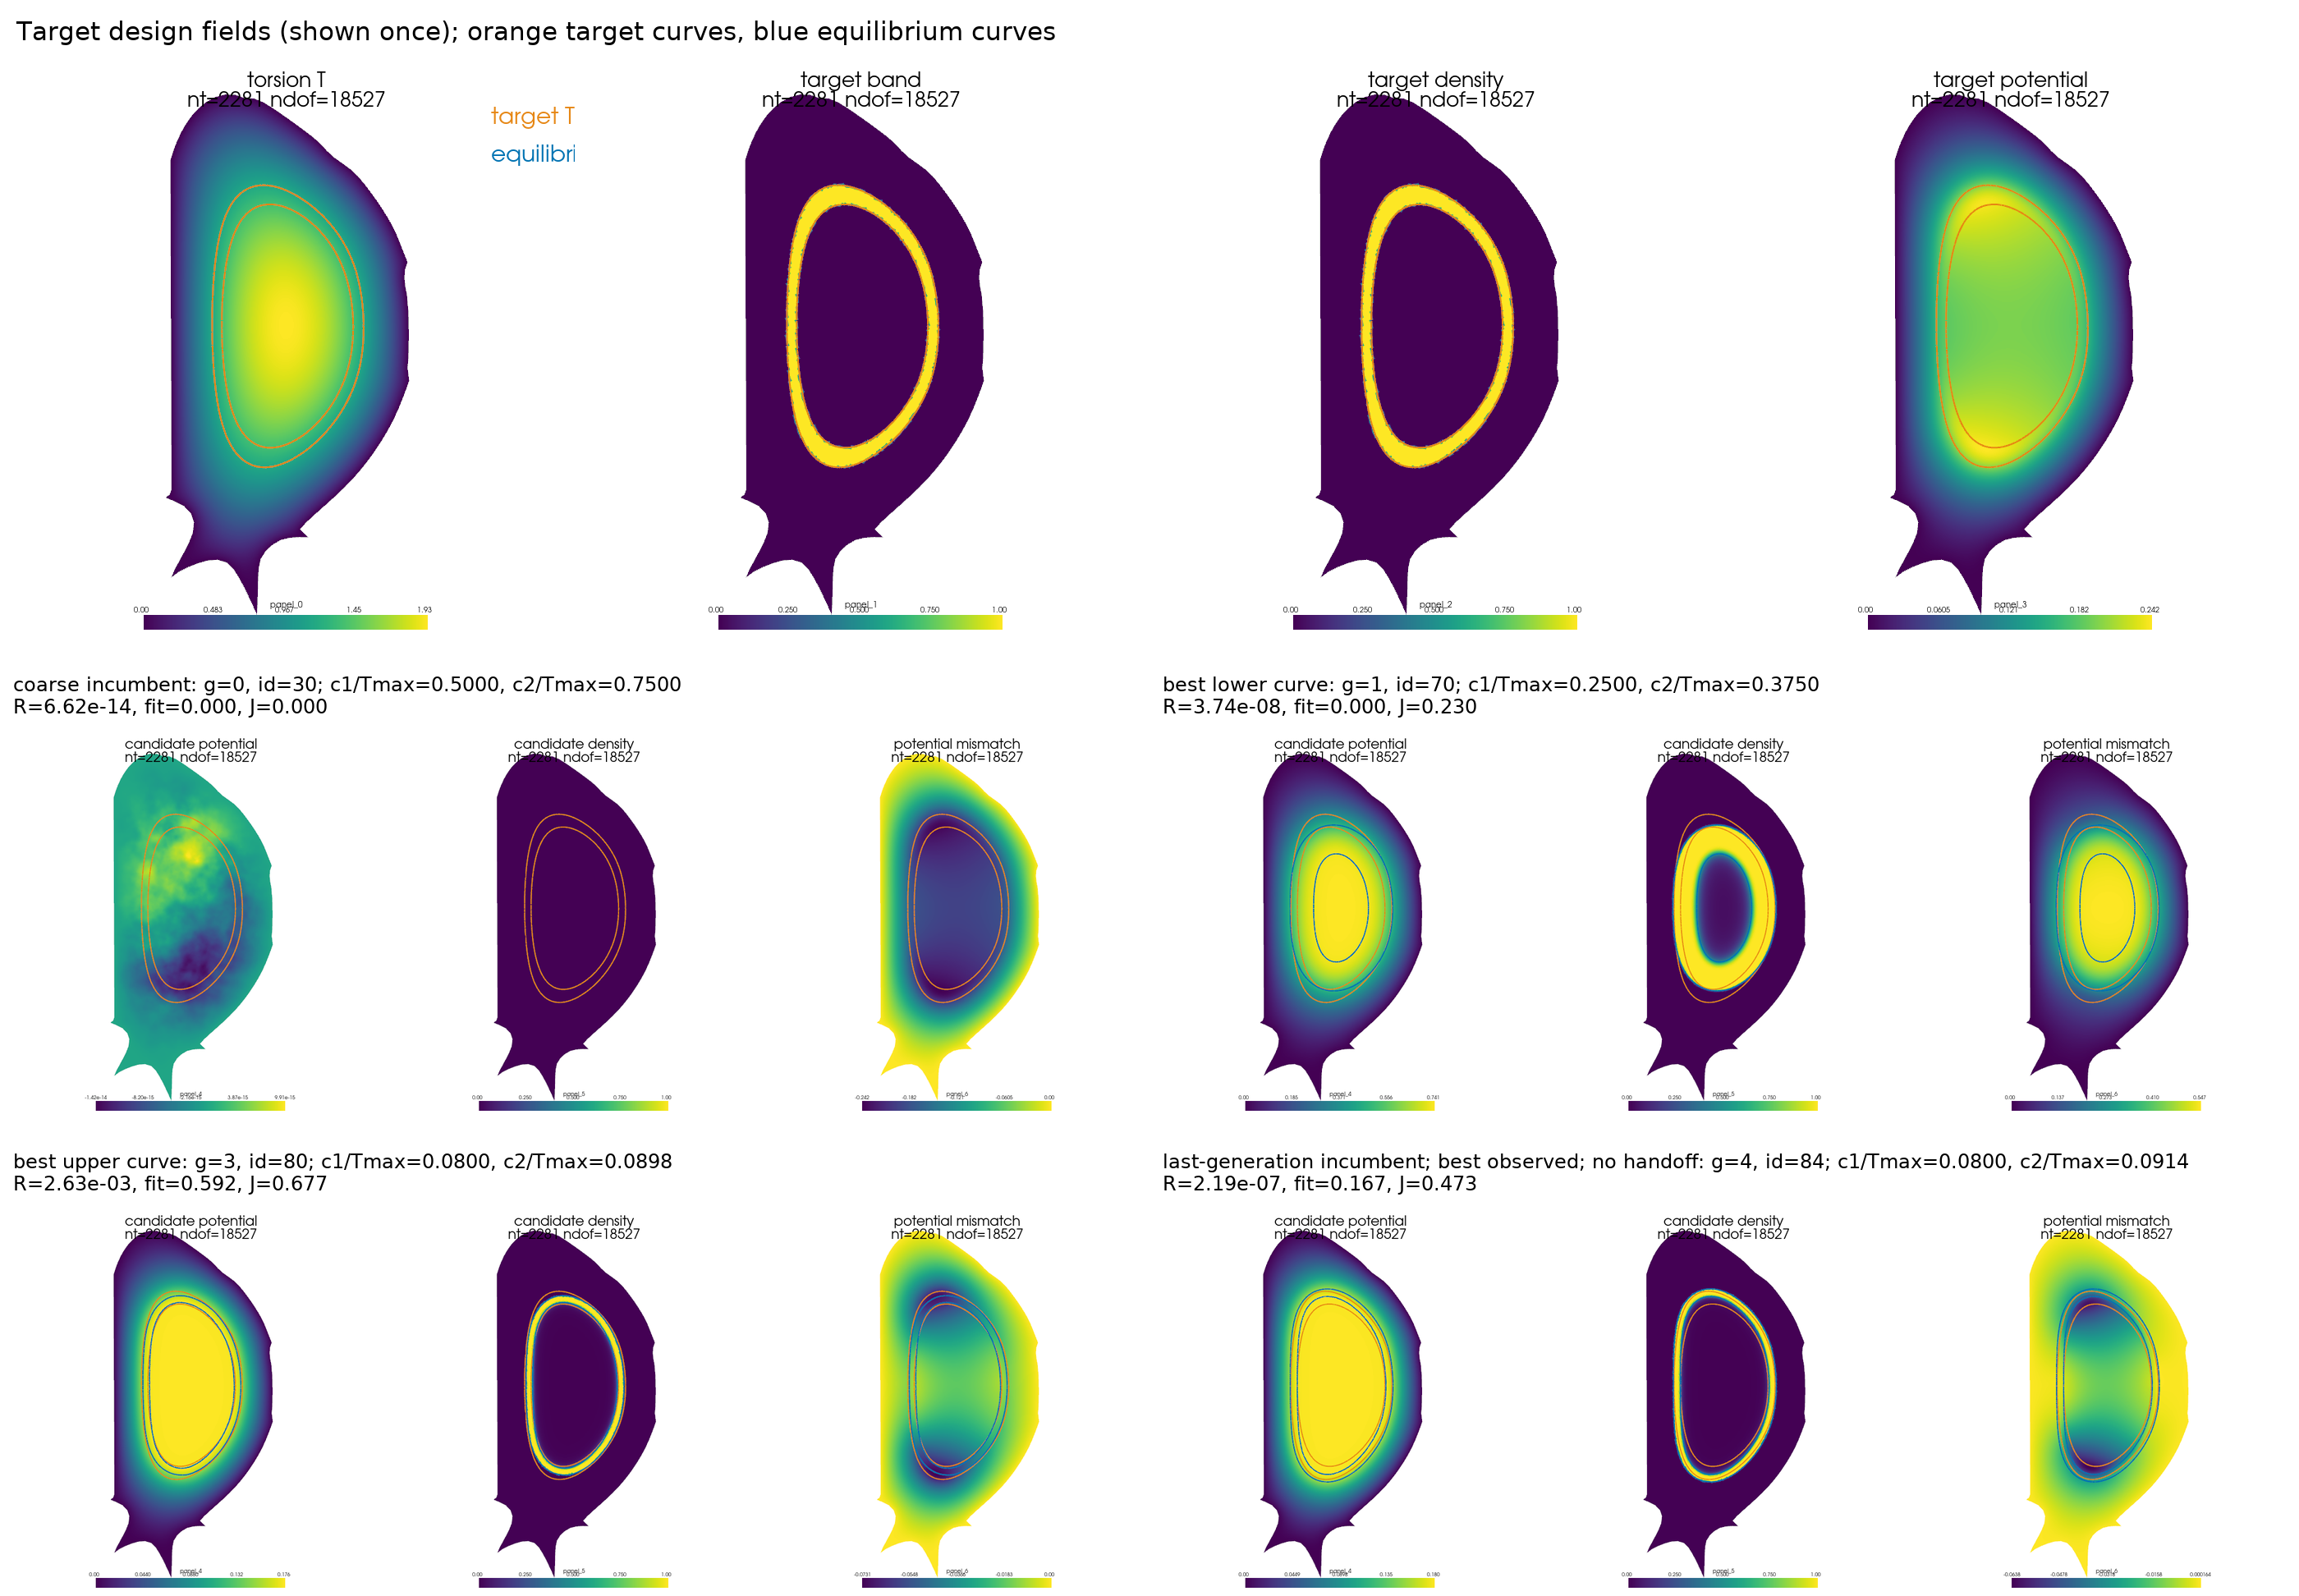
\includegraphics[width=\linewidth]{figures/iter_0p6_0p7_adaptive_continuation_eps002_lowdof_candidate_storyboard.png}
  \caption{Geometry-independent adaptive search for the ITER
  $[0.6,0.7]T_{\max}$ band. The target design fields are shown once in the
  first row; subsequent rows show candidate equilibria while retaining the
  dashed target-band contours for comparison. Candidate~80 is identified in
  the storyboard as the best upper-curve/hard-overlap candidate. The image
  records partial and failed candidates as well as PDE-qualified candidates,
  so geometric promise is not confused with nonlinear convergence.}
  \label{fig:iter-candidate80-adaptive-search}
\end{figure}

The suffix \texttt{eps002} in the search directory denotes the \emph{relative}
smoothing ratio $\varepsilon_\phi/\Delta c_\phi=0.02$, not the absolute value
$\varepsilon_\phi=0.002$. Since candidate~80 has
$\Delta c_\phi=0.0188843$, its search solve used
$\varepsilon_\phi=3.777\times10^{-4}$. At this sharp smoothing, Newton made
46 iterations before terminating with \texttt{FAIL\_LS} at
$2.628\times10^{-3}$. The state and pair were then handed directly to a
fixed-pair nonlinear solve---with no homotopy and no threshold update---using
the larger absolute smoothing $\varepsilon_\phi=0.003$. This is about
$7.94$ times the search smoothing and corresponds to
$\varepsilon_\phi/\Delta c_\phi\simeq0.159$.

The direct run used a sharp torsion target, a P4 space with 2,281 cells and
18,527 global degrees of freedom, quadrature degree 16, and MUMPS for the
linearized solves. The inner Newton tolerance was $10^{-6}$ and the final
projection tolerance was $10^{-10}$. Its saved nonlinear residual sequence
was
\[
  1.293\times10^{-2}\;\longrightarrow\;
  3.260\times10^{-3}\;\longrightarrow\;
  6.603\times10^{-4}\;\longrightarrow\;
  4.173\times10^{-5}\;\longrightarrow\;
  2.470\times10^{-7}\;\longrightarrow\;
  9.152\times10^{-12}.
\]
Thus the inner projection reached its requested tolerance without stalling,
and one final exact Newton update reduced the residual by a further factor of
approximately $2.7\times10^4$. Relative to the first saved fixed-smoothing
state, the final residual fell by approximately $1.4\times10^9$, i.e. more
than nine orders of magnitude.

\begin{figure}[p]
  \centering
  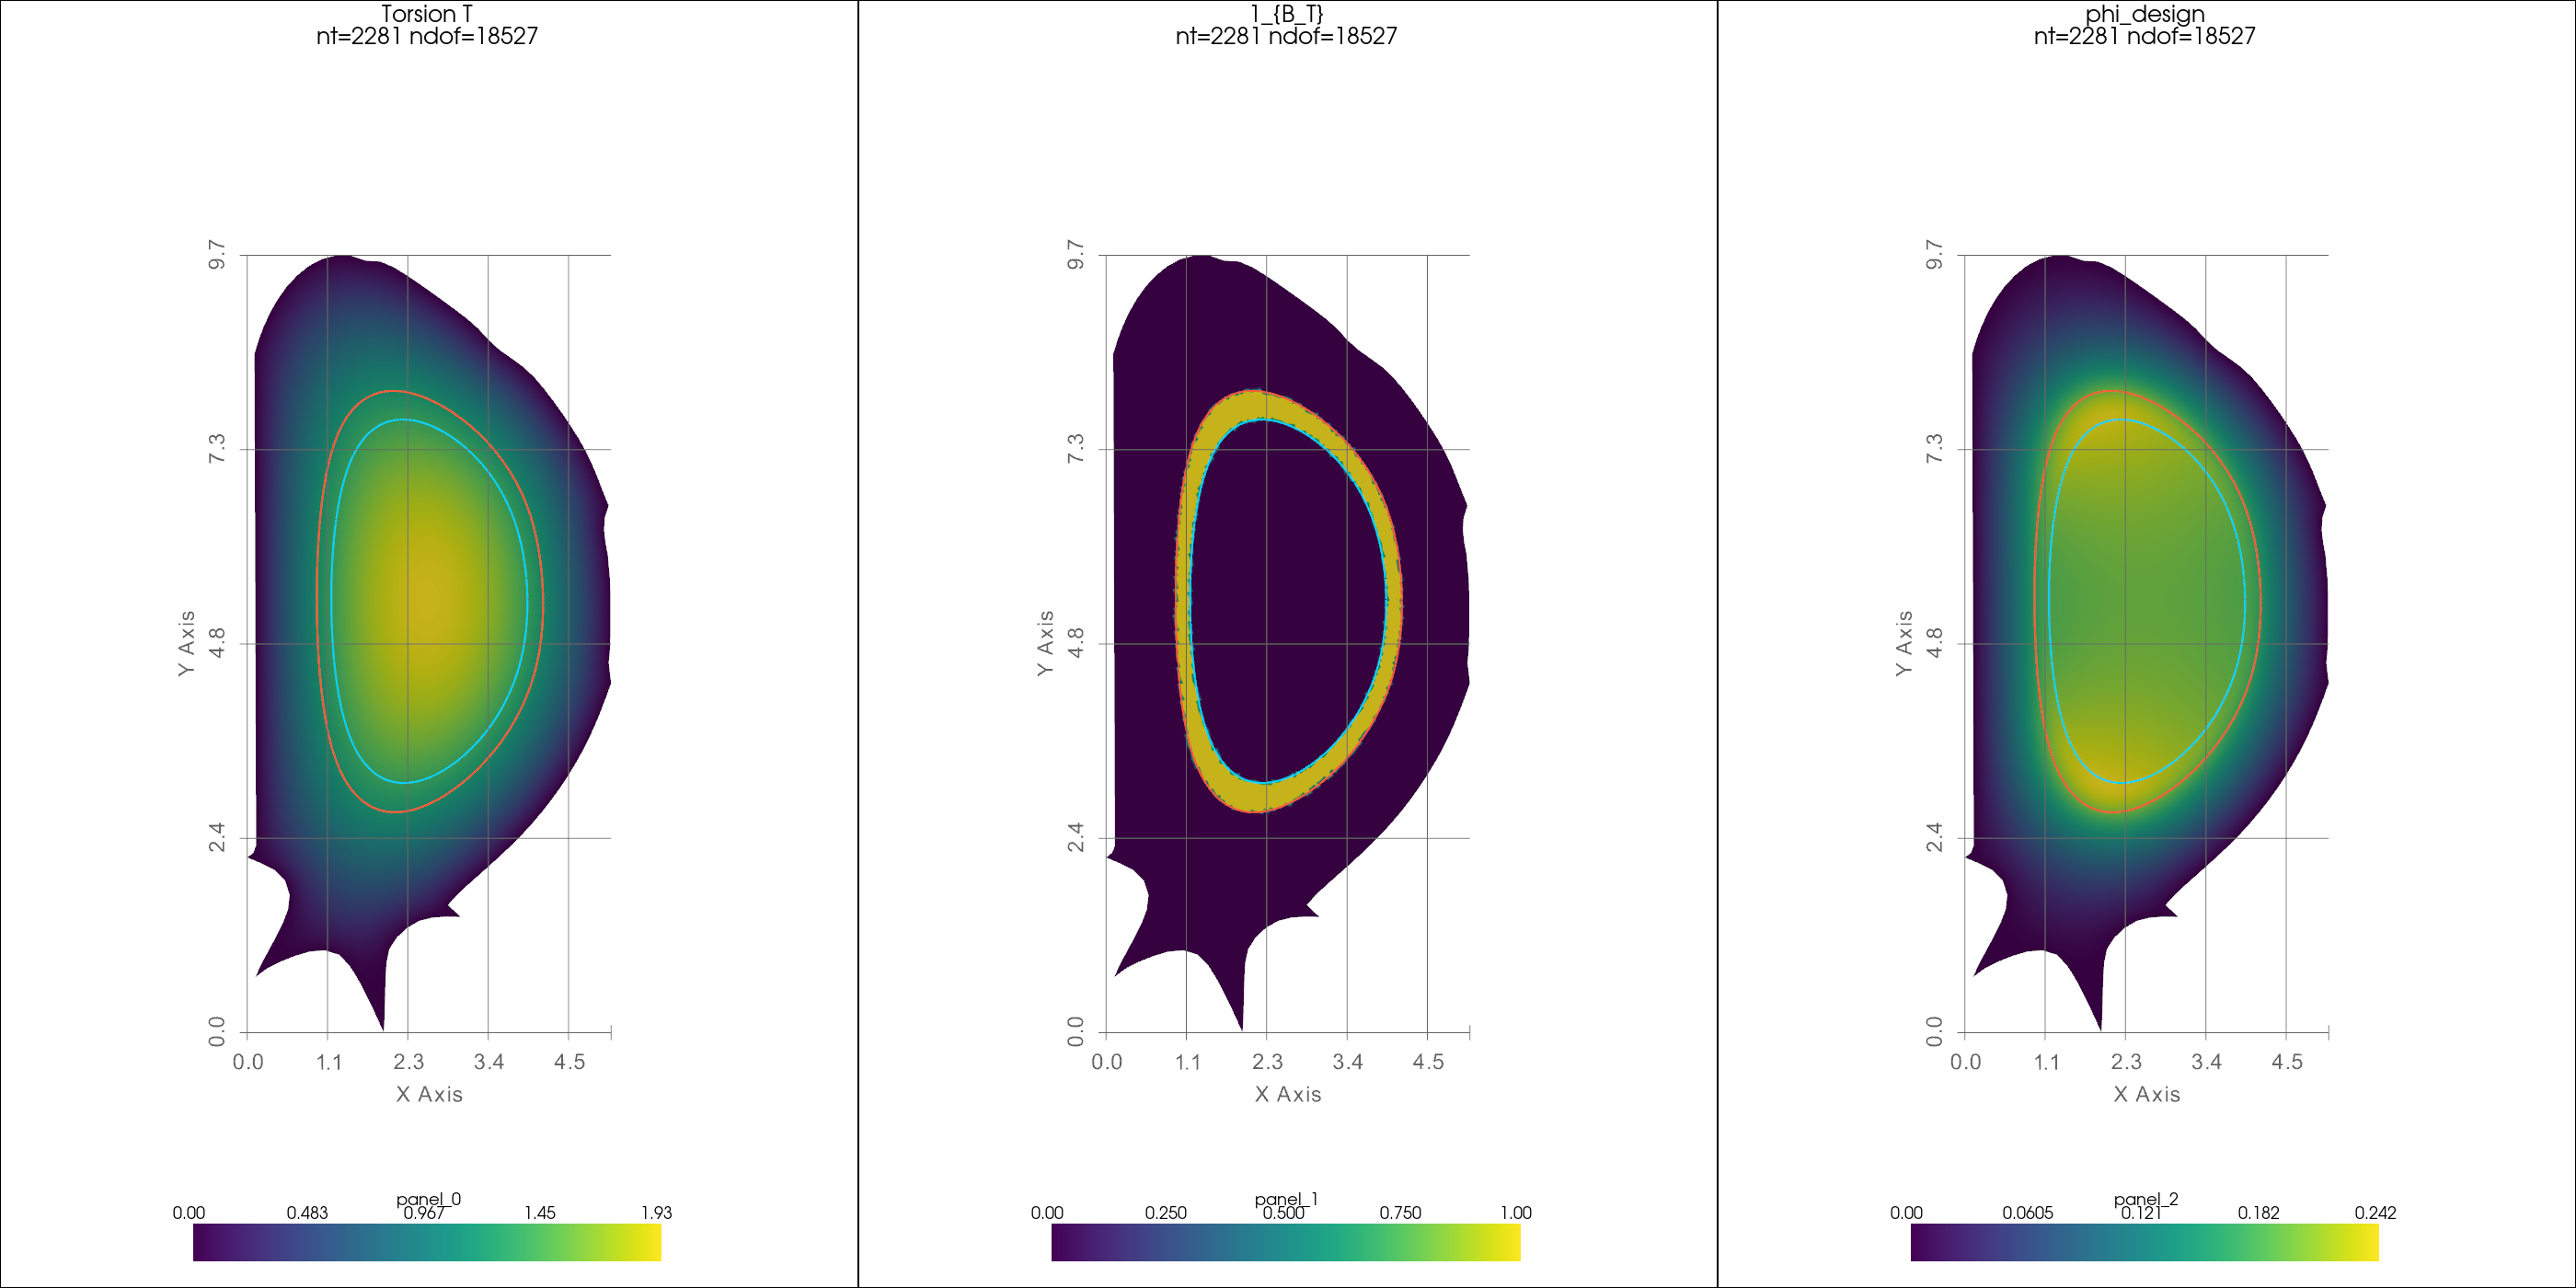
\includegraphics[width=0.96\linewidth,height=0.68\textheight,keepaspectratio]{figures/iter_candidate80_fixed_pair_eps0003_targets.png}
  \caption{Geometric target fields for the direct ITER handoff experiment:
  torsion $T$, the sharp target band $\rho_T$, and its Poisson potential
  $\phi_T$. The orange contours mark the prescribed
  $[0.6,0.7]T_{\max}$ band. The fixed targets are separated from the
  nonlinear evolution so that both figures remain legible.}
  \label{fig:iter-candidate80-fixed-targets}
\end{figure}

\begin{landscape}
\begin{figure}[p]
  \centering
  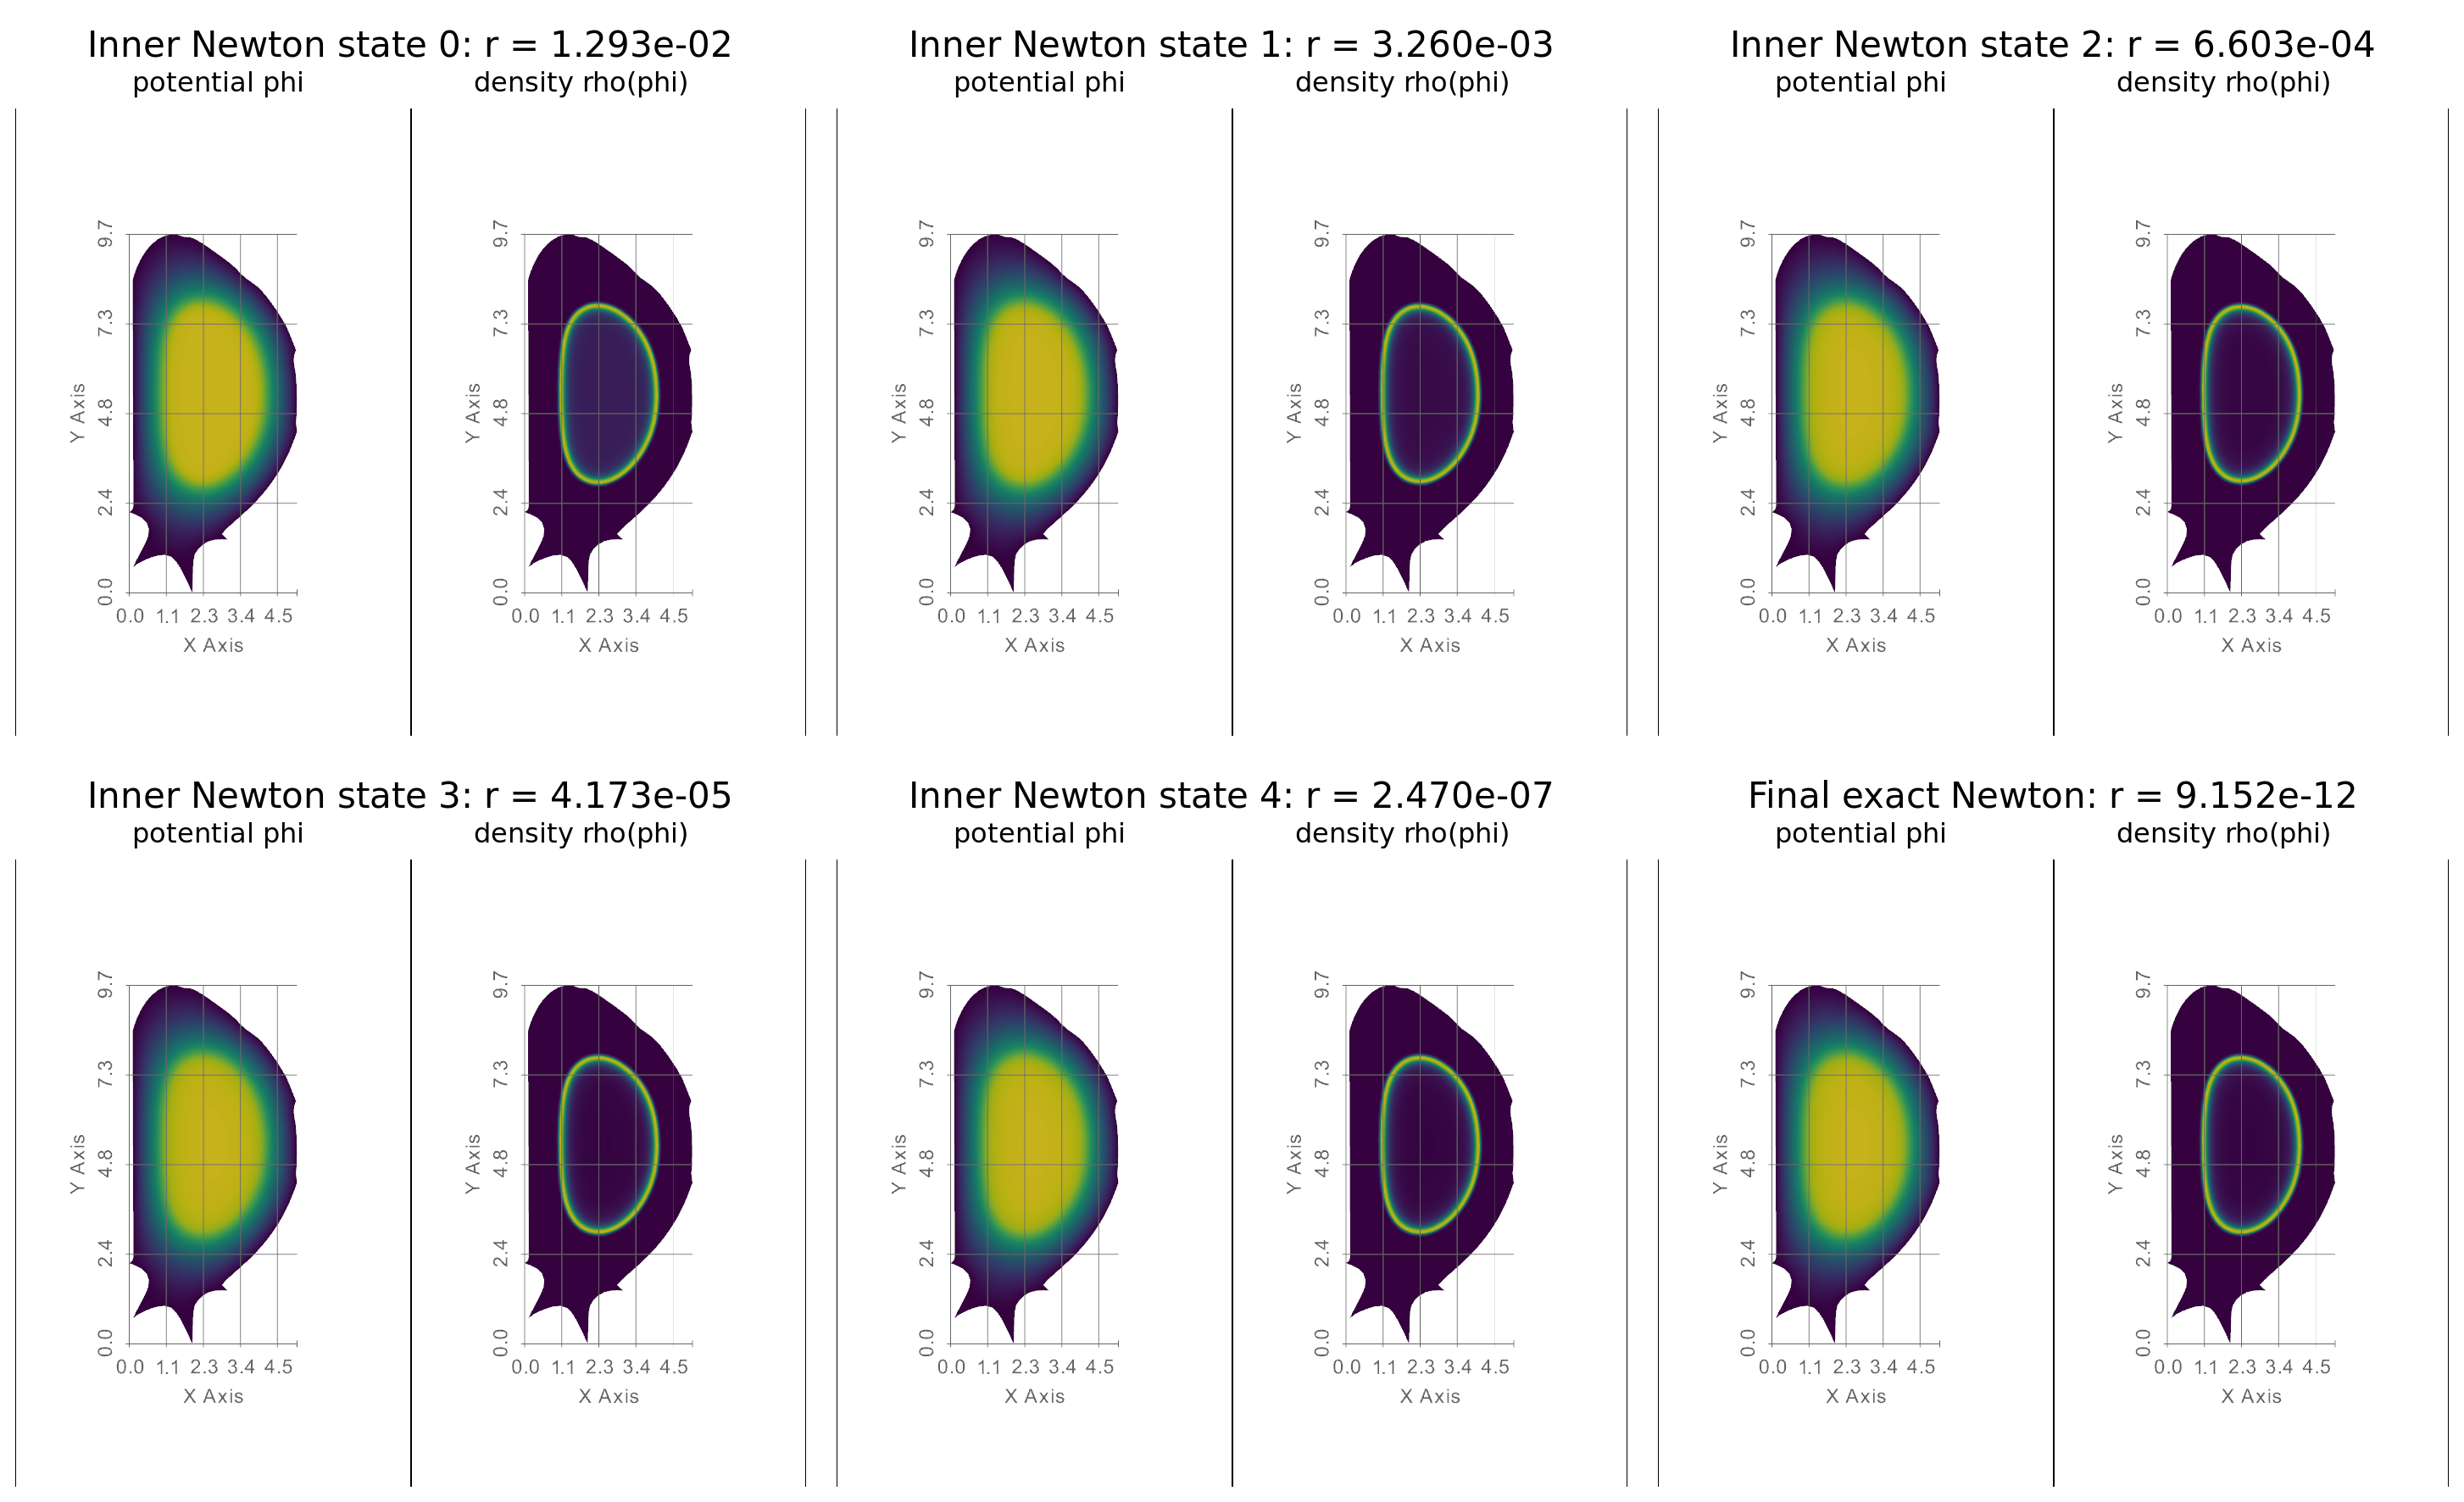
\includegraphics[width=0.96\linewidth,height=0.78\textheight,keepaspectratio]{figures/iter_candidate80_fixed_pair_eps0003_newton_storyboard.png}
  \caption{Direct, non-homotopy handoff of adaptive-search candidate~80 at
  fixed $(c_{1,\phi},c_{2,\phi})=(0.1547293,0.1736136)$ and
  $\varepsilon_\phi=0.003$. The five saved inner-Newton states and final
  exact projection form a $3\times2$ grid. Each snapshot shows the evolving
  potential $\phi$ and smoothed density $\rho(\phi)$; its label gives the
  Euclidean nonlinear residual. The fixed target fields appear separately in
  Figure~\ref{fig:iter-candidate80-fixed-targets}, and the residual sequence
  matches Table~\ref{tab:iter-candidate80-newton}.}
  \label{fig:iter-candidate80-fixed-handoff}
\end{figure}
\end{landscape}

\begin{table}[htbp]
  \centering
  \caption{Newton behavior for adaptive-search candidate~80 and its direct
  fixed-pair handoff. The search row and the handoff rows use the same
  thresholds but different smoothing. Iteration counts are the solver's
  reported counts; the storyboard stores accepted states rather than every
  trial or backtrack.}
  \label{tab:iter-candidate80-newton}
  \resizebox{\linewidth}{!}{%
  \begin{tabular}{@{}lrrrl@{}}
    \toprule
    phase & $\varepsilon_\phi$ & Newton iterations
      & terminal residual & nonlinear status \\
    \midrule
    adaptive-search candidate
      & $0.02\Delta c_\phi=3.777\times10^{-4}$
      & 46 & $2.628\times10^{-3}$ & \texttt{FAIL\_LS} \\
    direct inner projection
      & $3.000\times10^{-3}$
      & 5 & $2.470\times10^{-7}$ & \texttt{CONVERGED\_RESIDUAL} \\
    final exact projection
      & $3.000\times10^{-3}$
      & 1 & $9.152\times10^{-12}$ & \texttt{CONVERGED\_RESIDUAL} \\
    \bottomrule
  \end{tabular}%
  }
\end{table}

The inner and final Newton calls reported $0.833\,\mathrm{s}$ and
$0.164\,\mathrm{s}$, respectively, whereas the complete diagnostic run took
$87.33\,\mathrm{s}$. This older run predates the detailed
\texttt{newton.csv} and \texttt{phases.csv} instrumentation; consequently,
the remaining time cannot be separated reliably into assembly, sensitivity,
geometric-diagnostic, plotting, and I/O costs, nor can rejected line-search
trials and damping factors be reconstructed. The available evidence does,
however, show that Newton itself was decisive and fast once the fixed
smoothing was enlarged: it converged monotonically through the saved states
and the final projection substantially exceeded the requested residual
tolerance.

Nonlinear convergence did not imply geometric convergence. At the converged
fixed-smoothing state, the active Jaccard index was $0.4191$, relative leakage
was $0.2429$, relative missing area was $0.4650$, and the active area was
$2.2973$ versus the target area $2.9533$ (an area ratio of $0.7779$). These
are worse than candidate~80's sharp-smoothing search metrics. Moreover, the
fixed-pair experiment accepted zero threshold-optimization steps; its outer
wrapper retained the label \texttt{MAX\_OPT\_IT}, but this label is not a
Newton failure. We therefore classify the experiment as a \emph{successful
state handoff and nonlinear PDE solve}, but not as strict geometric
convergence of the optimized band. The comparison isolates a genuine
trade-off: increasing $\varepsilon_\phi$ regularized the nonlinear solve, but
broadened the transition enough to degrade containment and active-set overlap.

\subsection{High-resolution direct fractional initialization for ITER}
\label{sec:iter-fractional-highdof}
We next tested a deliberately simpler initialization strategy on the same
ITER target band,
$0.6\,T_{\max}\leq T\leq0.7\,T_{\max}$. This diagnostic run did not use the
$L^2$/quantile window fit, the $H^{-1}$ search, or a homotopy stage. Instead,
it transferred the prescribed torsion fractions directly to the potential of
the target density,
\[
  (c_{1,\phi}^{(0)},c_{2,\phi}^{(0)})
  =(0.6,0.7)\,\|\phi_T\|_{L^\infty}
  =(0.14479650,0.16892925),
\]
where $\|\phi_T\|_{L^\infty}=0.24132750$. Thus the initialization used only
quantities computed for the current geometry and target; it was not supplied
with a previously successful equilibrium pair. This experiment is a
diagnostic exception to the homotopy-based production protocol described
above.

The mesh contained 24,430 triangular cells and the P4 discretization had
196,369 global degrees of freedom. Quadrature degree 16 was used. The sharp
torsion indicator was retained ($\varepsilon_T=0$), while the equilibrium
smoothing was fixed globally at $\varepsilon_\phi=0.003$. The run used eight
MPI ranks with one numerical-library thread per rank and MUMPS in the
nonlinear, sensitivity, and final-projection phases. Most importantly for
interpreting the reduced derivatives, the initial, trial, and final Newton
solves were all required to reach a residual tolerance of $10^{-12}$ before a
state could be accepted.

The direct seed was nonlinear-solver compatible. Its nine Newton updates gave
the residual history
\[
\begin{aligned}
  2.715\!\times\!10^{-2}&\to2.423\!\times\!10^{-2}
  \to1.257\!\times\!10^{-2}\to7.436\!\times\!10^{-3}
  \to1.361\!\times\!10^{-3}\\
  &\to2.712\!\times\!10^{-5}\to1.319\!\times\!10^{-7}
  \to3.288\!\times\!10^{-12}\to2.436\!\times\!10^{-14}.
\end{aligned}
\]
Consequently, the reduced optimization began from a fully converged PDE
state, rather than using an inexact initial Newton iterate. The projected
seed nevertheless had only moderate geometric agreement: its active Jaccard
index was $0.3965$, with relative leakage $0.8389$ and relative missing area
$0.7854$.

\begin{landscape}
\begin{figure}[p]
  \centering
  \begin{minipage}{\linewidth}
  \centering
  \captionsetup{width=\linewidth}
  \captionsetup[subfigure]{font=scriptsize,skip=1pt}
  \makebox[\linewidth][c]{%
  \begin{subfigure}[t]{0.18\linewidth}
    \centering
    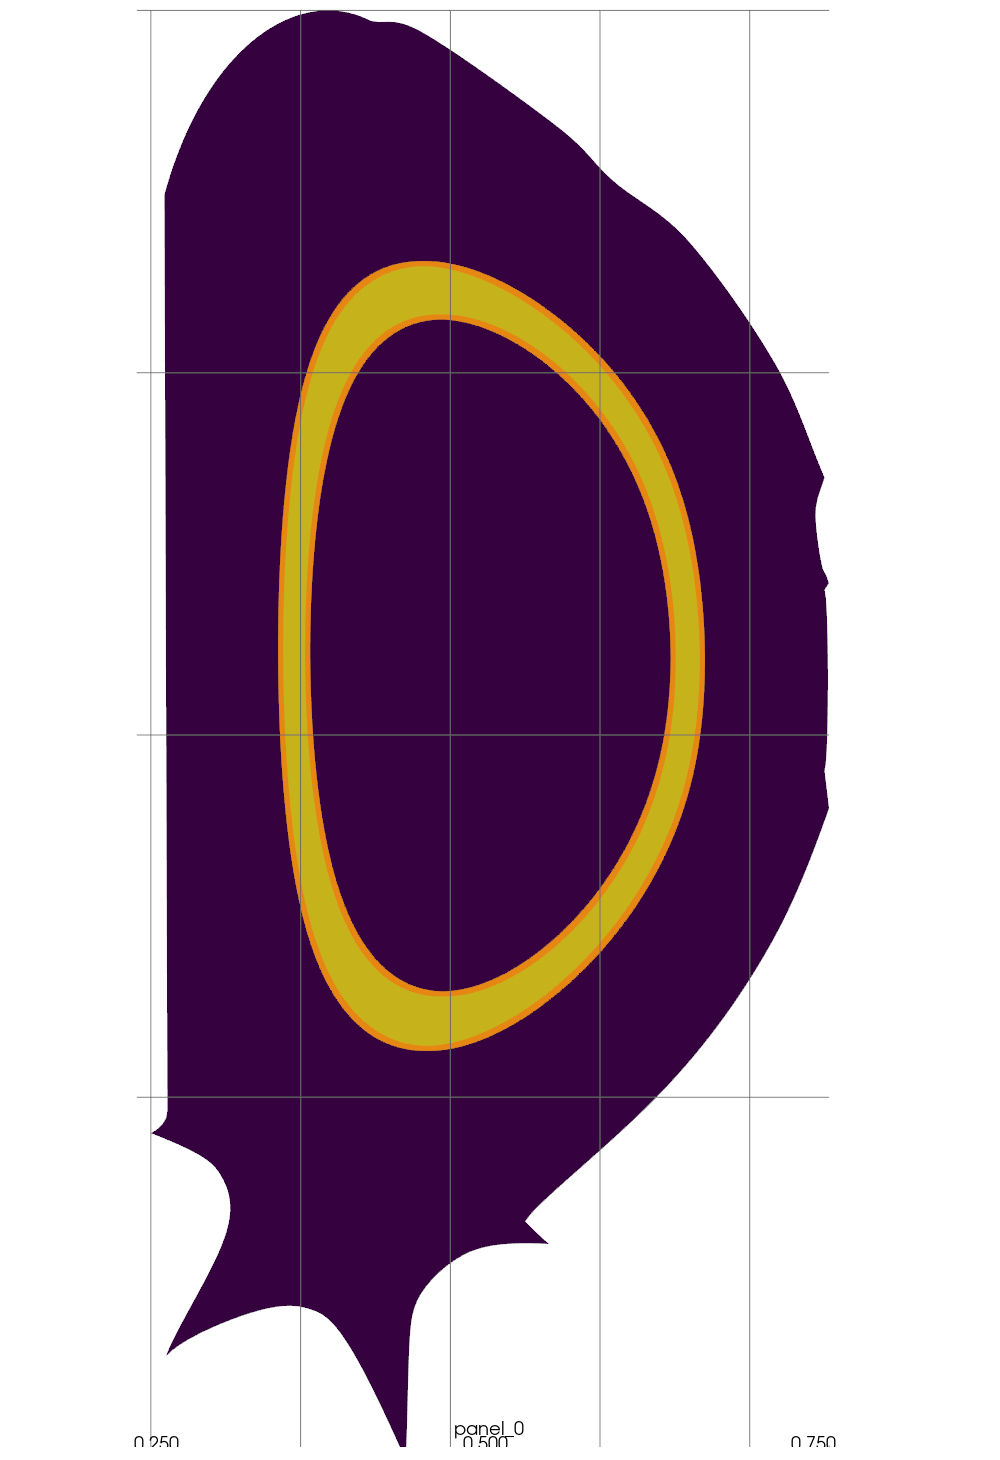
\includegraphics[width=\linewidth,height=0.35\textheight,keepaspectratio]{figures/iter_0p6_0p7_fractional_highdof_panel_01_target.png}
    \caption{Target design}
  \end{subfigure}%
  \hspace{0.01\linewidth}%
  \begin{subfigure}[t]{0.18\linewidth}
    \centering
    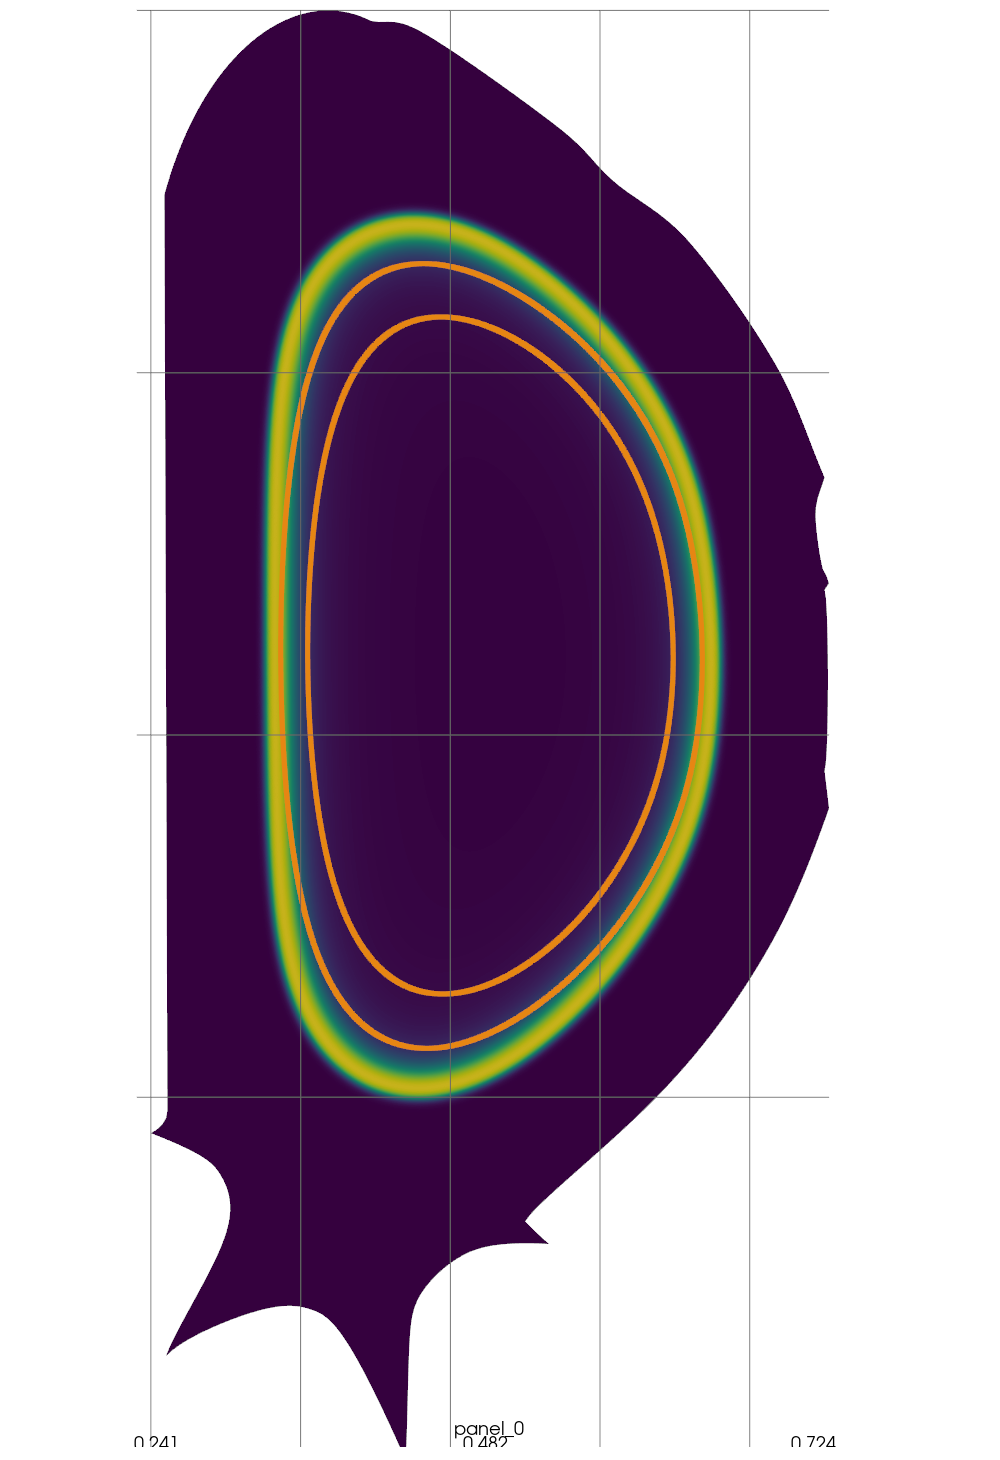
\includegraphics[width=\linewidth,height=0.35\textheight,keepaspectratio]{figures/iter_0p6_0p7_fractional_highdof_panel_02_seed.png}
    \caption{Projected direct seed}
  \end{subfigure}%
  \hspace{0.01\linewidth}%
  \begin{subfigure}[t]{0.18\linewidth}
    \centering
    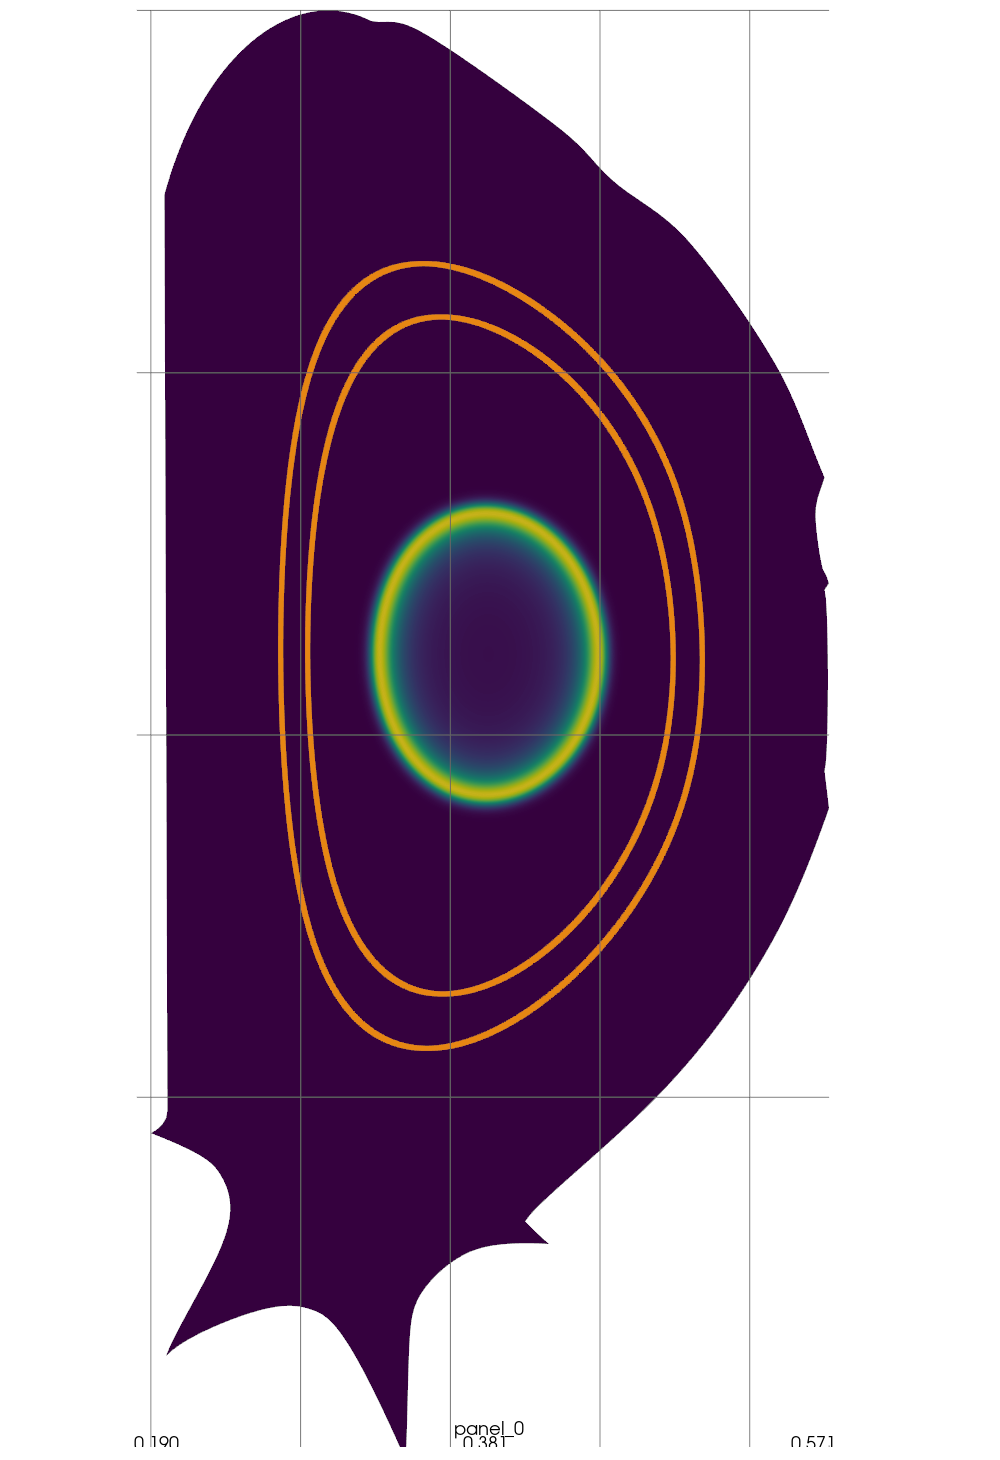
\includegraphics[width=\linewidth,height=0.35\textheight,keepaspectratio]{figures/iter_0p6_0p7_fractional_highdof_panel_03_rejected_k0.png}
    \caption{Rejected central band, $k=0$}
  \end{subfigure}%
  \hspace{0.01\linewidth}%
  \begin{subfigure}[t]{0.18\linewidth}
    \centering
    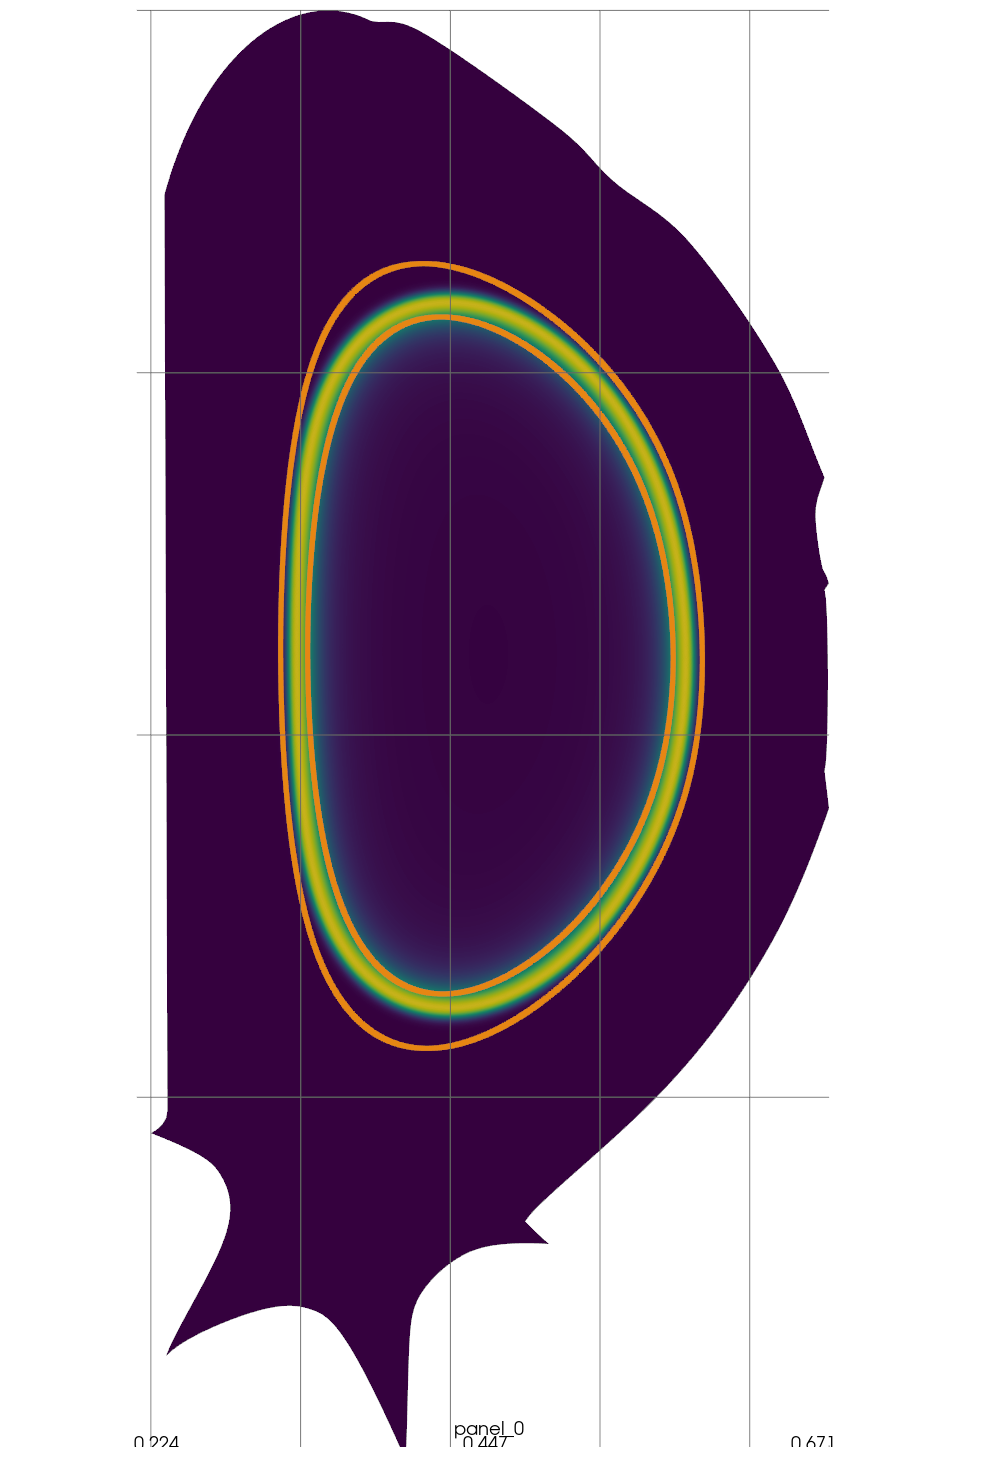
\includegraphics[width=\linewidth,height=0.35\textheight,keepaspectratio]{figures/iter_0p6_0p7_fractional_highdof_panel_04_accept_k1.png}
    \caption{First recovery, $k=1$}
  \end{subfigure}}

  \vspace{1mm}

  \makebox[\linewidth][c]{%
  \begin{subfigure}[t]{0.18\linewidth}
    \centering
    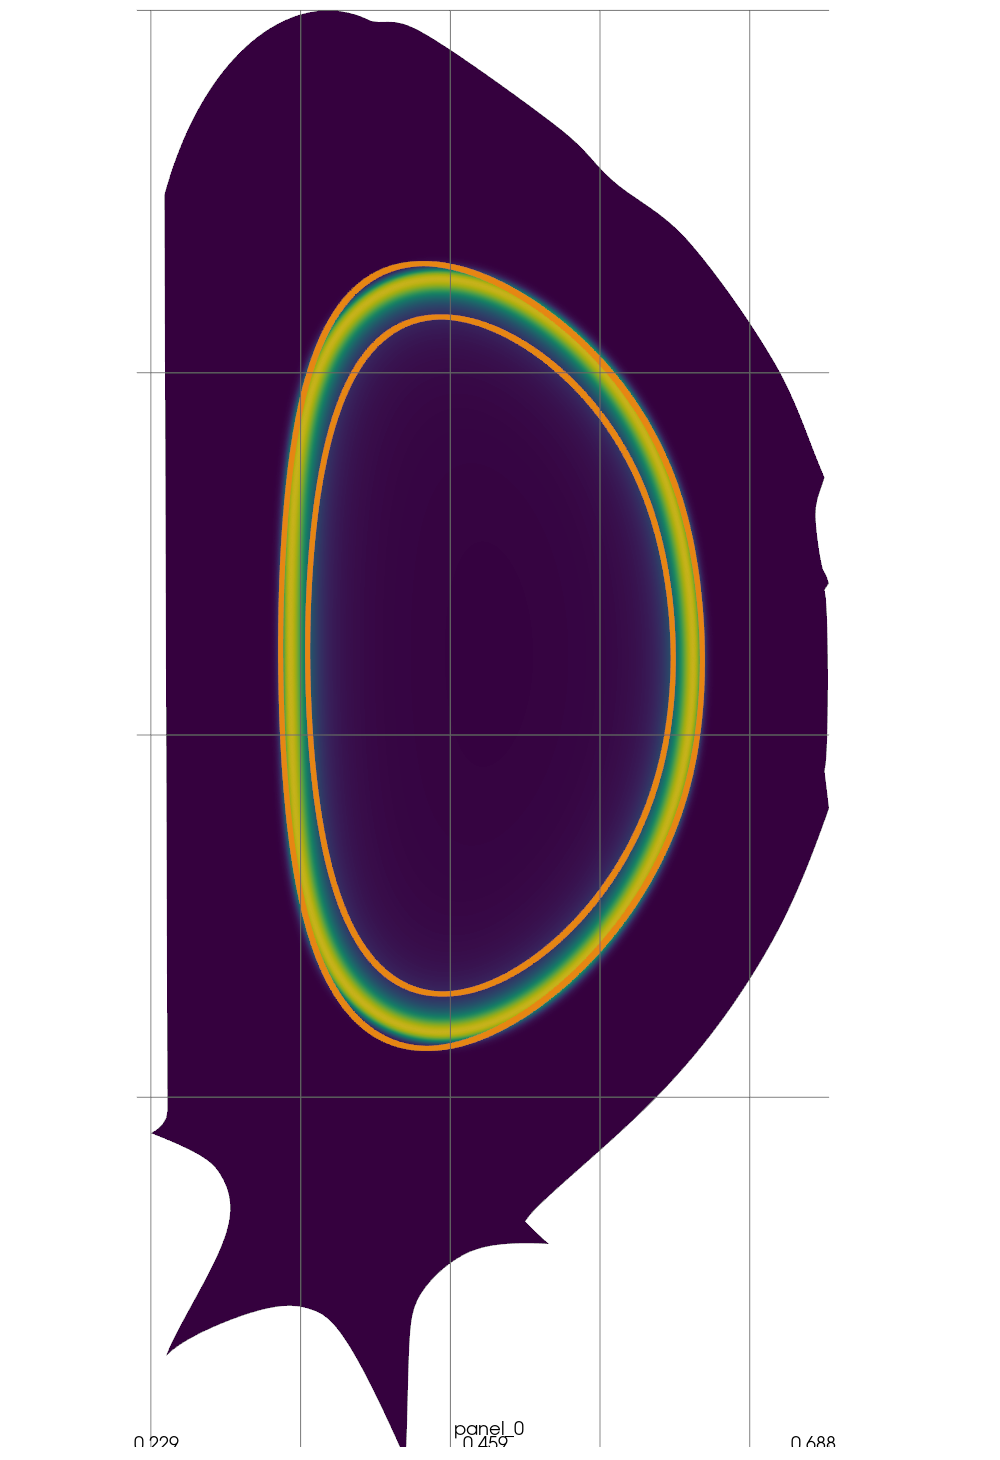
\includegraphics[width=\linewidth,height=0.35\textheight,keepaspectratio]{figures/iter_0p6_0p7_fractional_highdof_panel_05_best_k5.png}
    \caption{Best Jaccard, $k=5$}
  \end{subfigure}%
  \hspace{0.01\linewidth}%
  \begin{subfigure}[t]{0.18\linewidth}
    \centering
    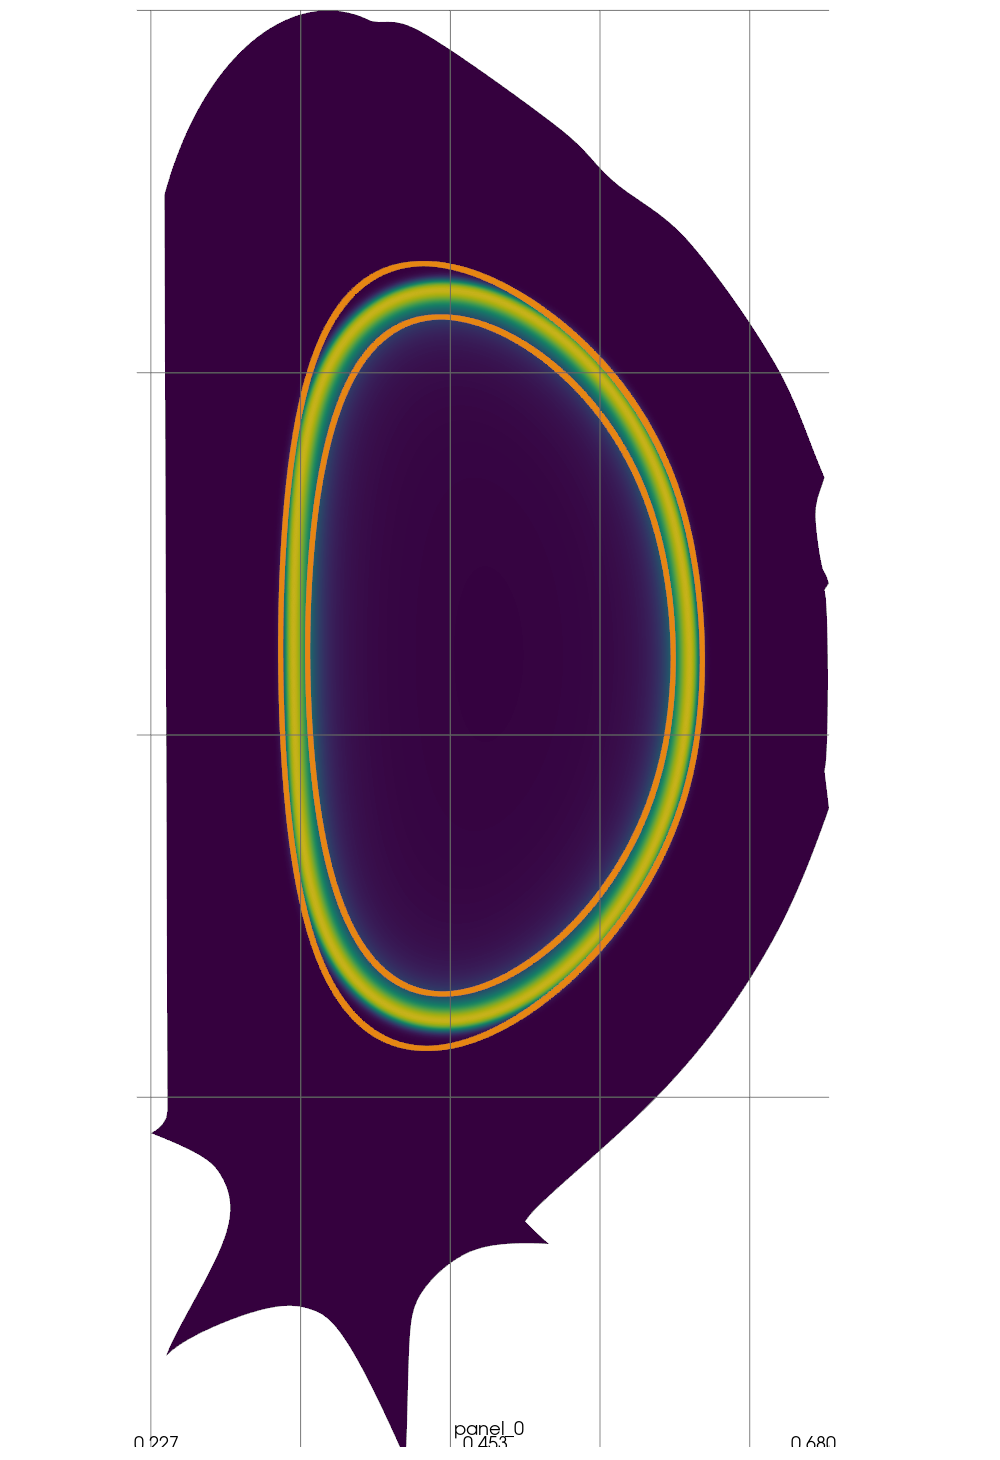
\includegraphics[width=\linewidth,height=0.35\textheight,keepaspectratio]{figures/iter_0p6_0p7_fractional_highdof_panel_06_accept_k7.png}
    \caption{Accepted state, $k=7$}
  \end{subfigure}%
  \hspace{0.01\linewidth}%
  \begin{subfigure}[t]{0.18\linewidth}
    \centering
    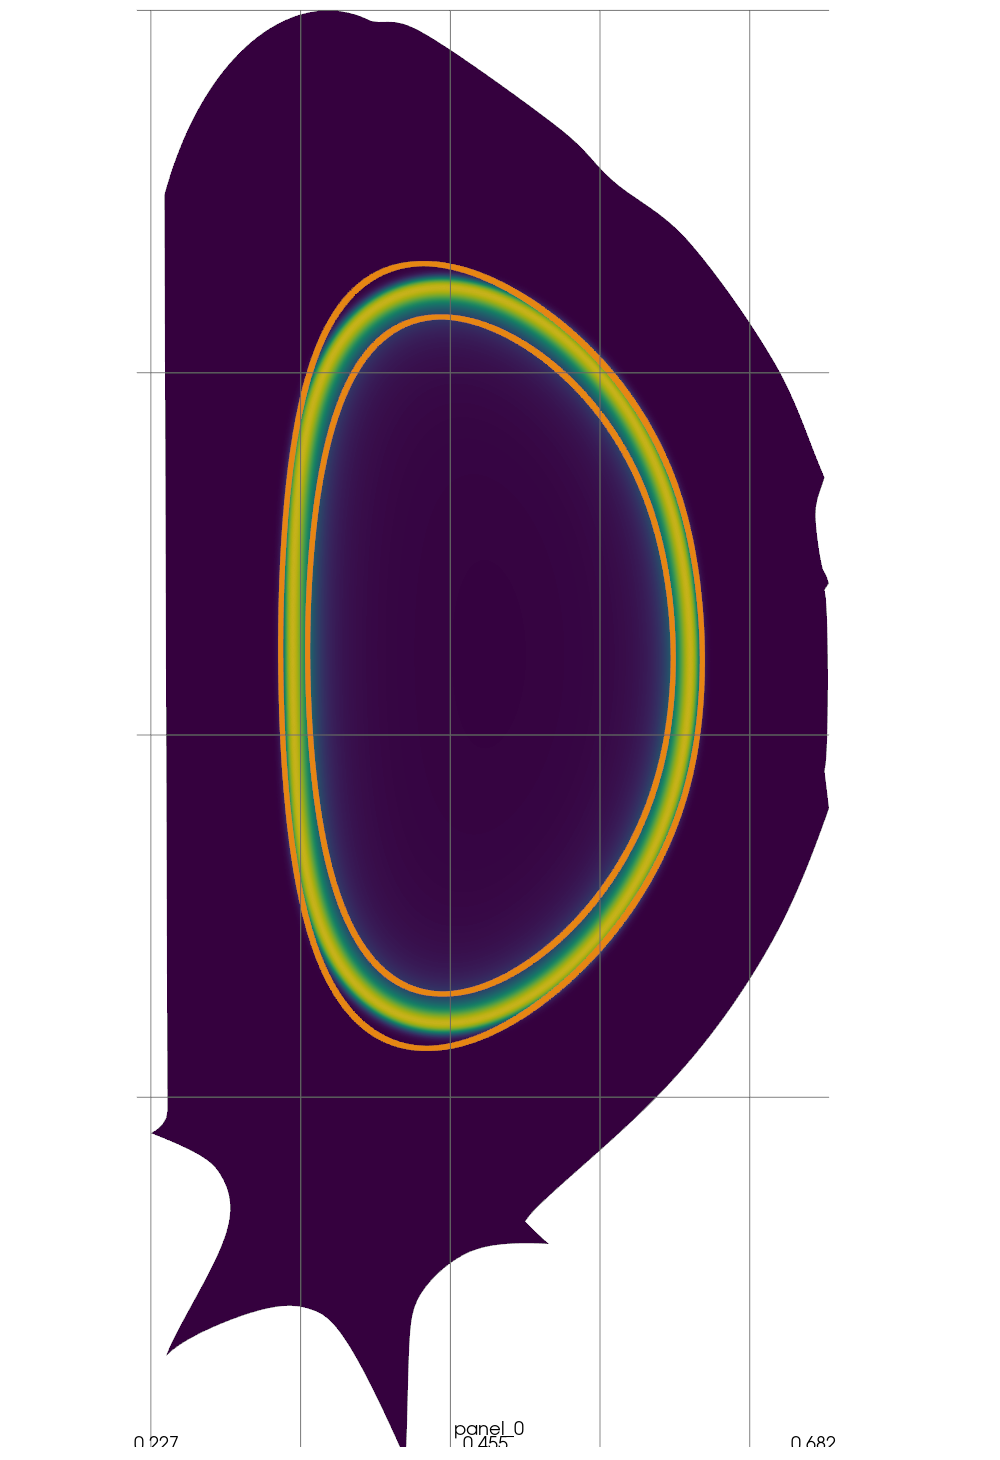
\includegraphics[width=\linewidth,height=0.35\textheight,keepaspectratio]{figures/iter_0p6_0p7_fractional_highdof_panel_07_accept_k11.png}
    \caption{Accepted state, $k=11$}
  \end{subfigure}%
  \hspace{0.01\linewidth}%
  \begin{subfigure}[t]{0.18\linewidth}
    \centering
    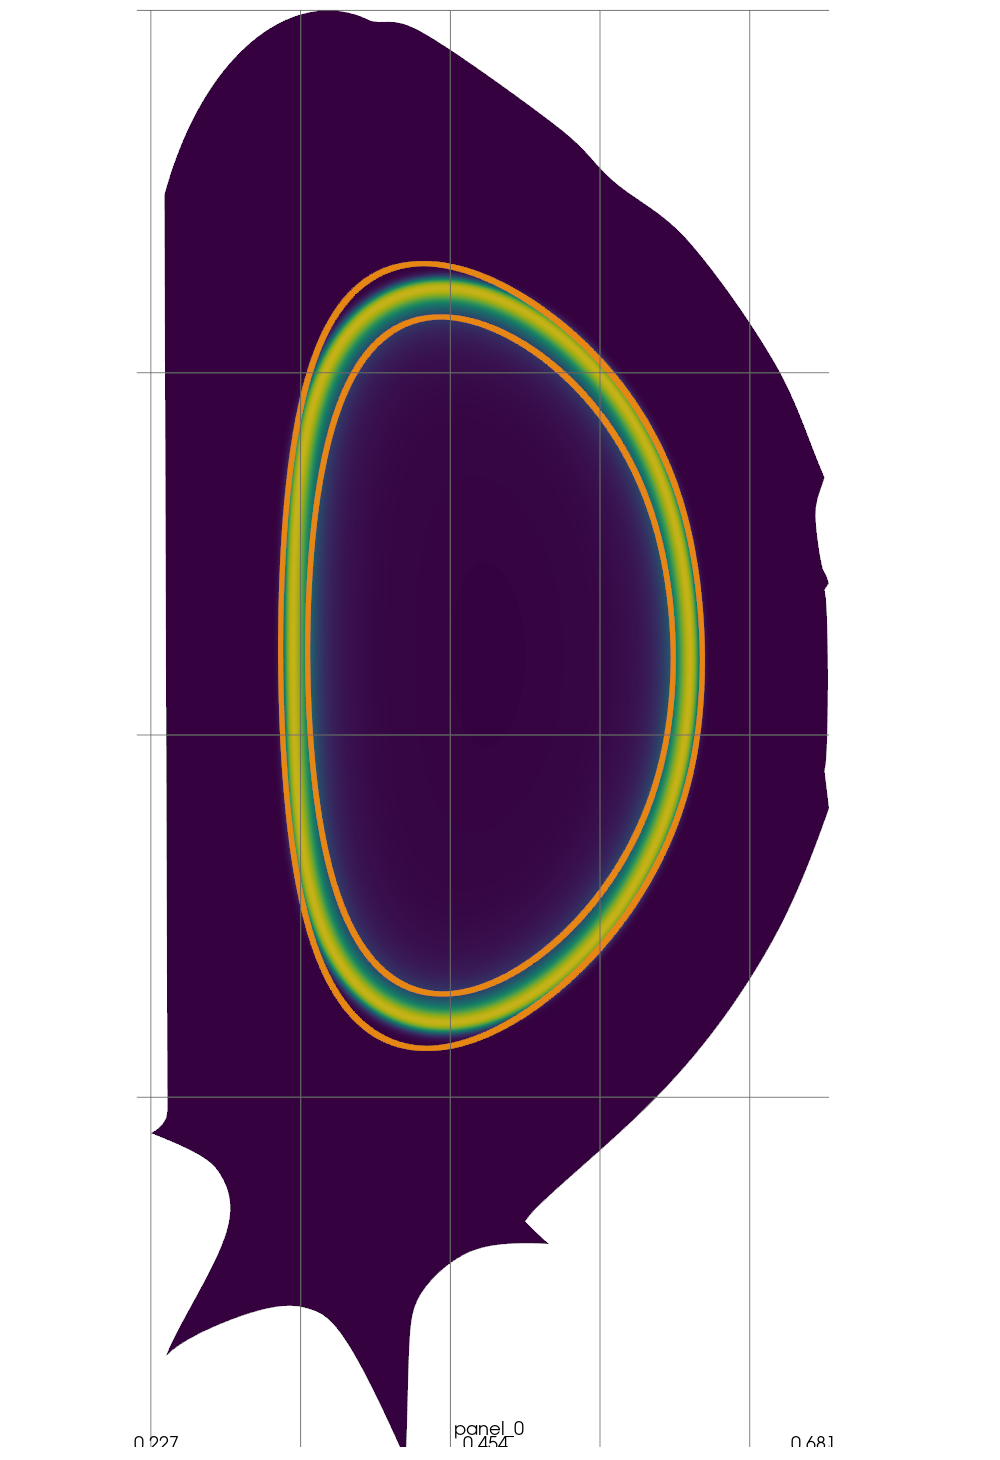
\includegraphics[width=\linewidth,height=0.35\textheight,keepaspectratio]{figures/iter_0p6_0p7_fractional_highdof_panel_08_final.png}
    \caption{Final step-floor state}
  \end{subfigure}}
  \caption{High-resolution ITER evolution under direct fractional
  initialization. The fixed target design is shown only once; every
  subsequent panel shows the equilibrium density with the prescribed torsion
  band retained as orange dashed contours. The sequence includes the fully
  projected seed, the rejected minimum-width central-band excursion at
  $k=0$, the first accepted recovery, the best active-Jaccard state at $k=5$,
  two later accepted states, and the final state. No mesh edges are drawn, so
  the 196,369-DOF resolution does not obscure the density field.}
  \label{fig:iter-fractional-highdof-storyboard}
  \end{minipage}
\end{figure}
\end{landscape}

The first reduced trial exposes an important failure mode. At $k=0$ the
projected step proposed
$(c_{1,\phi},c_{2,\phi})=(0.15168432,0.16368432)$, whose width was exactly the
enforced lower bound $0.012$. Qualitatively, this pair collapsed the active
set to a small band near the centre of the domain. Quantitatively, its
Newton residual first decreased from $6.326\times10^{-2}$ to approximately
$1.64\times10^{-3}$, but then stagnated as line-search damping fell from
order one to $3.64\times10^{-12}$. The trial ended in
\texttt{FAIL\_LS} after 62 Newton updates, with residual
$1.643\times10^{-3}$; its relative missing area was essentially one and its
branch-overlap score was only $0.0049$. The strict PDE and branch gates
therefore rejected it. This was the correct acceptance decision, although
substantial nonlinear work had already been spent resolving an evidently bad
threshold pair.

Trust-region contraction then moved the thresholds back to the geometrically
relevant branch. The first accepted recovery, at $k=1$, used
$(0.14860176,0.16594544)$ and converged in ten Newton updates to
$1.302\times10^{-13}$. After three further rejected trial pairs, $k=5$
accepted $(0.14774759,0.16661936)$ and attained the largest observed active
Jaccard index, $0.5128$, at residual $2.267\times10^{-14}$. Accepted updates
also occurred at $k=7$, 11, and 14. Every accepted trial was fully Newton
converged, so the nonmonotone geometric history cannot be attributed to
evaluating threshold sensitivities on unresolved PDE states.

\begin{figure}[p]
  \centering
  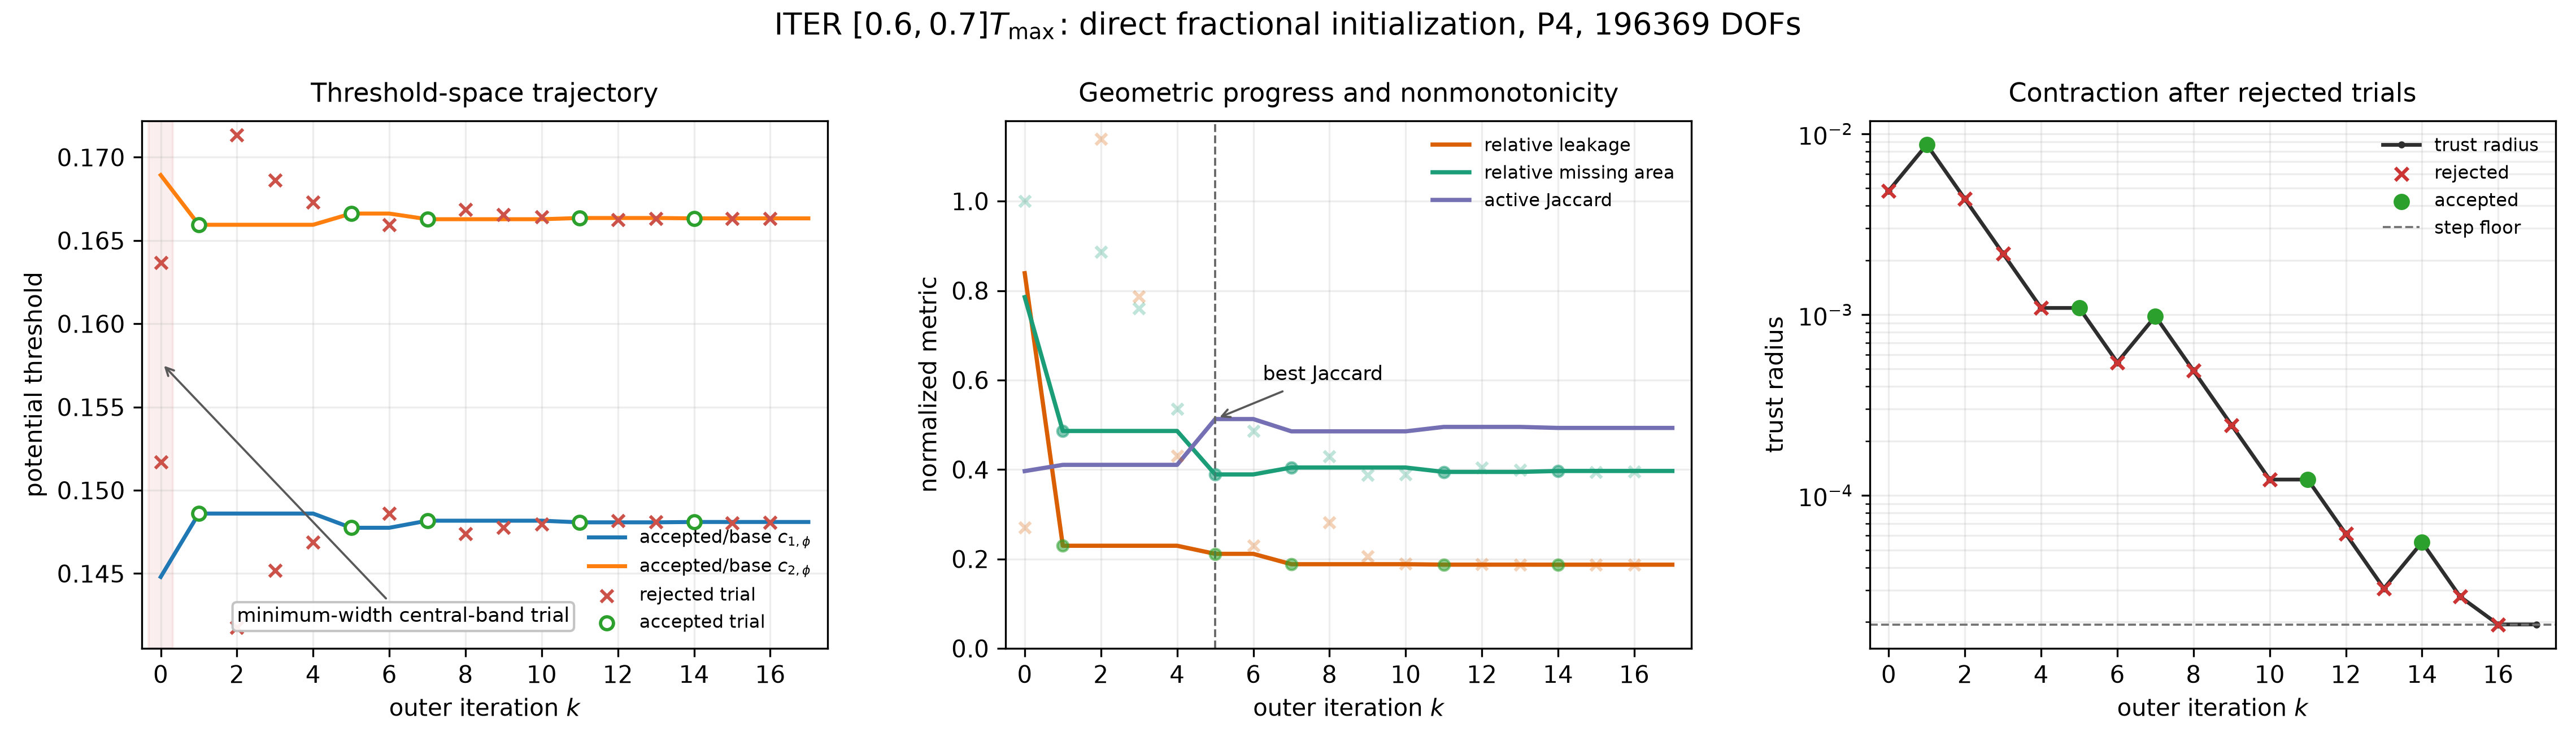
\includegraphics[width=\linewidth]{figures/iter_0p6_0p7_fractional_highdof_optimization_trace.png}
  \caption{Threshold-space and geometric history for the high-resolution
  direct-initialization run. Left: accepted/base thresholds and rejected
  trial pairs; the shaded first step is the minimum-width central-band
  excursion. Centre: relative leakage, relative missing area, and active
  Jaccard index at the accepted states, including the nonmonotone decrease
  after the best state at $k=5$. Right: trust-radius contraction caused by
  rejected trials and eventual contact with the step floor.}
  \label{fig:iter-fractional-highdof-trace}
\end{figure}

\begin{table}[htbp]
  \centering
  \caption{Selected fully converged states from the high-resolution direct
  fractional-initialization experiment. $L_{\rm rel}$ and $M_{\rm rel}$
  denote relative leakage and relative missing area, respectively. The best
  active-set overlap occurred before the final accepted threshold pair.}
  \label{tab:iter-fractional-highdof}
  \resizebox{\linewidth}{!}{%
  \begin{tabular}{@{}lrrrrrr@{}}
    \toprule
    state & $c_{1,\phi}$ & $c_{2,\phi}$ & residual
      & $L_{\rm rel}$ & $M_{\rm rel}$ & active Jaccard \\
    \midrule
    projected direct seed
      & 0.144797 & 0.168929 & $2.436\times10^{-14}$
      & 0.8389 & 0.7854 & 0.3965 \\
    first accepted recovery ($k=1$)
      & 0.148602 & 0.165945 & $1.302\times10^{-13}$
      & 0.2296 & 0.4862 & 0.4104 \\
    best Jaccard state ($k=5$)
      & 0.147748 & 0.166619 & $2.267\times10^{-14}$
      & 0.2115 & 0.3890 & 0.5128 \\
    final accepted state ($k=14$)
      & 0.148095 & 0.166330 & $7.584\times10^{-14}$
      & 0.1873 & 0.3968 & 0.4930 \\
    \bottomrule
  \end{tabular}%
  }
\end{table}

The threshold iteration terminated with \texttt{STEP\_TOO\_SMALL} after 18
outer records, comprising five accepted and twelve rejected trial pairs. At
the final pair the trust radius had contracted to
$1.934\times10^{-5}$ while the projected-gradient norm remained $3.97$.
The final exact Newton projection required no additional update because the
current residual, $7.584\times10^{-14}$, already exceeded the requested PDE
accuracy. Hence \texttt{STEP\_TOO\_SMALL} is a threshold-space termination,
not a Newton failure.

The final density captured most of the target band in the recall sense:
active recall was $0.9530$, active precision $0.5053$, and the corresponding
Dice coefficient $0.6604$. Its active area was $2.3416$ versus target area
$2.9622$, or $79.05\%$ of the target. The certified core was leakage-free,
but its area was only $0.6019$ ($20.32\%$ of the target); at the final width
$\Delta c_\phi=0.018235$, the fixed smoothing corresponds to
$\varepsilon_\phi/\Delta c_\phi\simeq0.1645$, leaving a relatively narrow
certified subband for $\kappa=2$.

The accepted Jaccard sequence was
$0.3965,0.4104,0.5128,0.4854,0.4953,0.4930$. The best state at $k=5$ was not
restored: only five steps had been accepted, fewer than the six required to
activate the configured Jaccard-stagnation test, and the final stale count was
three rather than the required four. We therefore classify this run as an
excellent nonlinear equilibrium solve with useful but partial geometric
capture, not as strict or certified-subband geometric convergence. It also
suggests a concrete efficiency safeguard for future runs: a topology/width
gate should reject a proposed minimum-width central band before committing to
a long fully converged Newton solve, while the best geometrically admissible
accepted state should be retained independently of the stopping trigger.

\clearpage
\subsection{No-homotopy direct fractional initialization for the lower ITER band}
\label{sec:iter-fractional-0p4-0p5}
We repeated the direct fractional-initialization experiment for the lower
ITER torsion band
$0.4\,T_{\max}\leq T\leq0.5\,T_{\max}$ with the script
\begin{center}
  \small
  \texttt{scripts/diocotron\_dolfinx/}\\[-0.2ex]
  \texttt{dolfinx\_torsion\_fractional\_phi\_target\_window\_}\\[-0.2ex]
  \texttt{reduced\_optimization.py}
\end{center}
As in Section~\ref{sec:iter-fractional-highdof}, the run used neither an
$L^2$/quantile fit nor an $H^{-1}$ threshold search, and it was not supplied
with a previous equilibrium. The target potential had
$\|\phi_T\|_{L^\infty}=0.16350845$, giving the direct seed
\[
  (c_{1,\phi}^{(0)},c_{2,\phi}^{(0)})
  =(0.4,0.5)\,\|\phi_T\|_{L^\infty}
  =(0.06540338,0.08175422).
\]
For this saved execution the direct Newton projection succeeded, so no source
homotopy was used. In particular, the recorded initialization contains only
direct Newton states and no homotopy stage.

The discretization and nonlinear accuracy matched the preceding
high-resolution ITER test: 24,430 triangular cells, a P4 space with 196,369
global degrees of freedom, quadrature degree 16, a sharp target indicator
($\varepsilon_T=0$), and fixed equilibrium smoothing
$\varepsilon_\phi=0.003$. Eight MPI ranks, one numerical-library thread per
rank, and MUMPS were used. Initial, trial, and final states were required to
satisfy the residual tolerance $10^{-12}$.

The direct seed converged without continuation. Its twelve saved Newton
updates had the residual history
\[
\begin{aligned}
  2.804\!\times\!10^{-2}&\to1.869\!\times\!10^{-2}
  \to1.432\!\times\!10^{-2}\to1.174\!\times\!10^{-2}\\
  &\to7.241\!\times\!10^{-3}\to5.021\!\times\!10^{-3}
  \to3.959\!\times\!10^{-3}\to2.642\!\times\!10^{-3}\\
  &\to4.333\!\times\!10^{-5}\to7.416\!\times\!10^{-7}
  \to1.432\!\times\!10^{-11}\to1.418\!\times\!10^{-14}.
\end{aligned}
\]
Thus the reduced derivatives were first evaluated on a fully resolved
nonlinear state. The projected seed was geometrically broad: its relative
leakage was $0.9365$, its relative missing area was $0.8523$, and its active
Jaccard index was $0.2690$.

\begin{landscape}
\begin{figure}[p]
  \centering
  \begin{minipage}{\linewidth}
  \centering
  \captionsetup{width=\linewidth}
  \captionsetup[subfigure]{font=scriptsize,skip=1pt}
  \makebox[\linewidth][c]{%
  \begin{subfigure}[t]{0.18\linewidth}
    \centering
    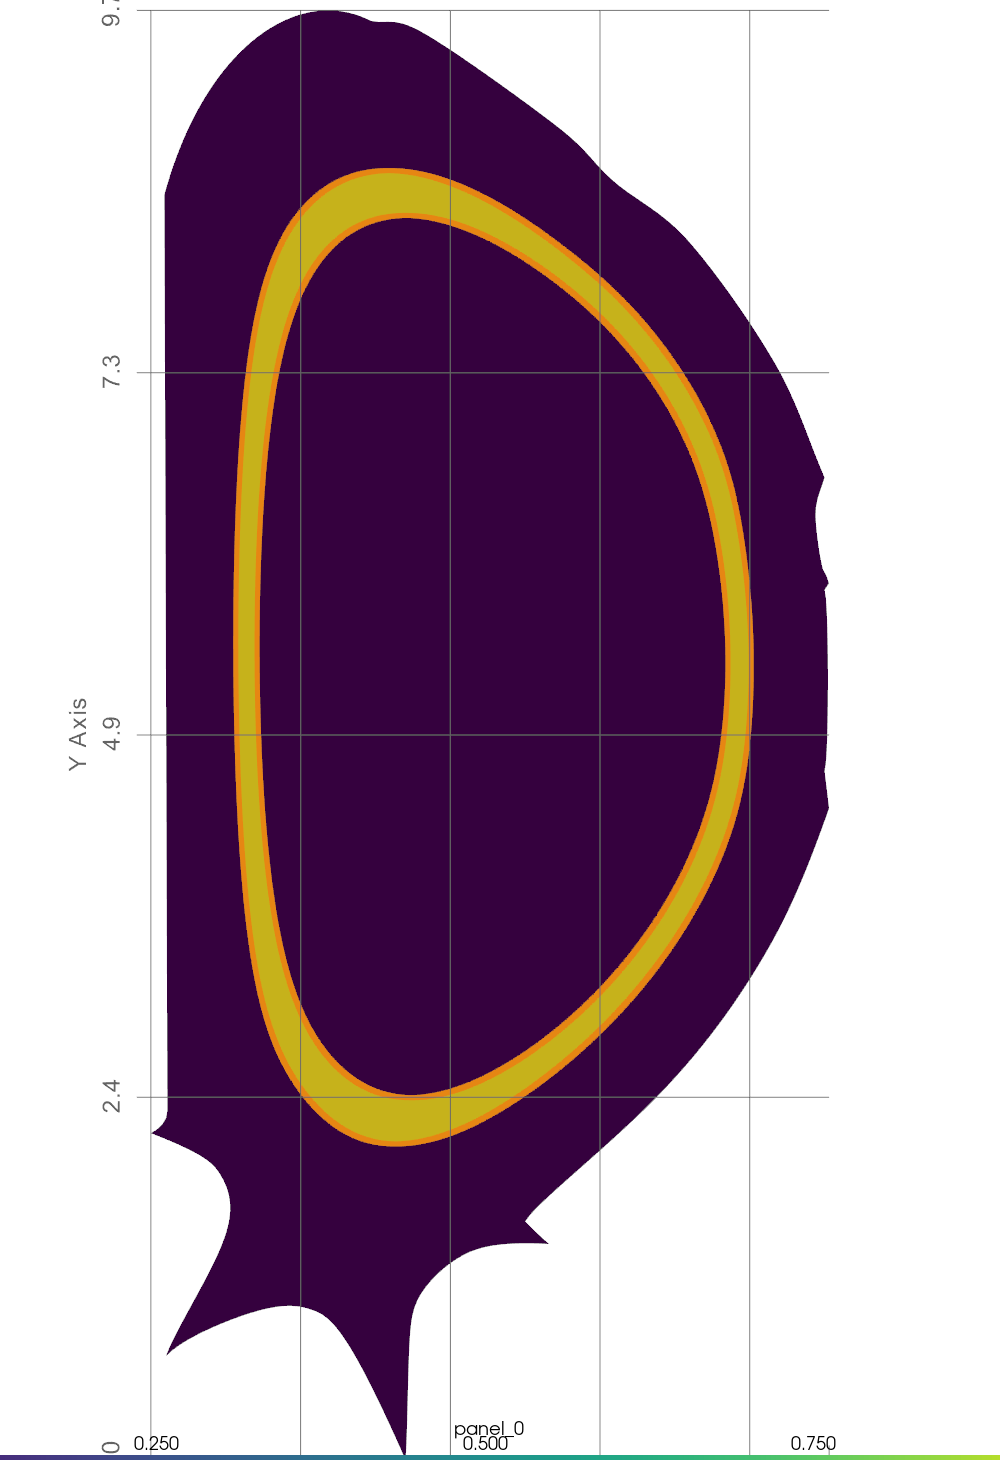
\includegraphics[width=\linewidth,height=0.35\textheight,keepaspectratio]{figures/iter_0p4_0p5_fractional_highdof_panel_01_target.png}
    \caption{Target design}
  \end{subfigure}%
  \hspace{0.01\linewidth}%
  \begin{subfigure}[t]{0.18\linewidth}
    \centering
    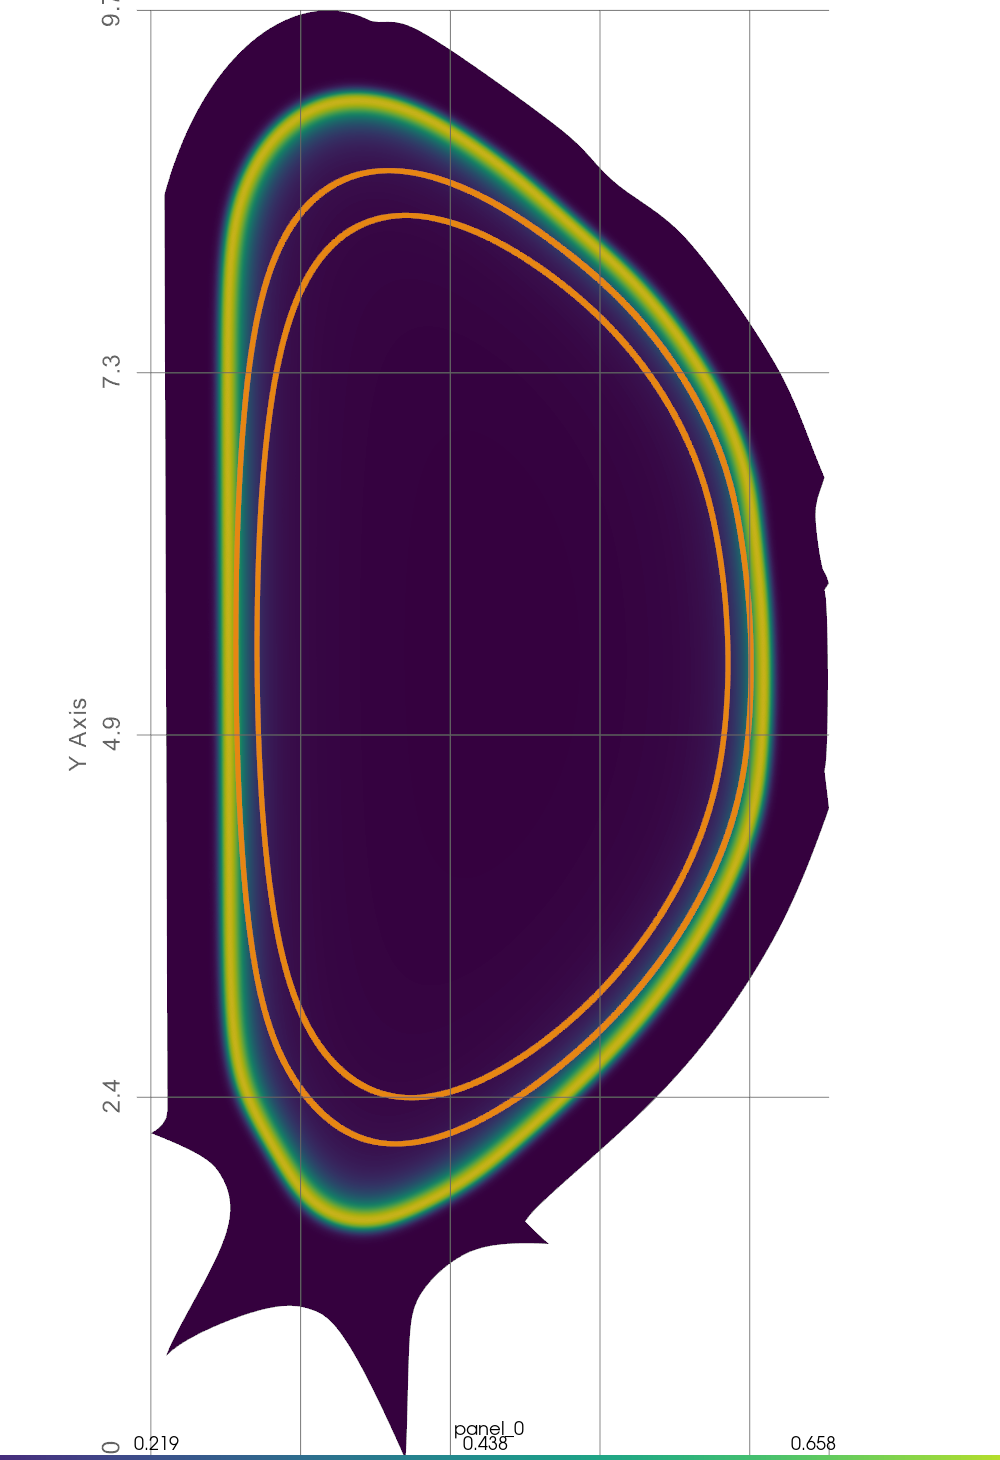
\includegraphics[width=\linewidth,height=0.35\textheight,keepaspectratio]{figures/iter_0p4_0p5_fractional_highdof_panel_02_seed.png}
    \caption{Projected direct seed}
  \end{subfigure}%
  \hspace{0.01\linewidth}%
  \begin{subfigure}[t]{0.18\linewidth}
    \centering
    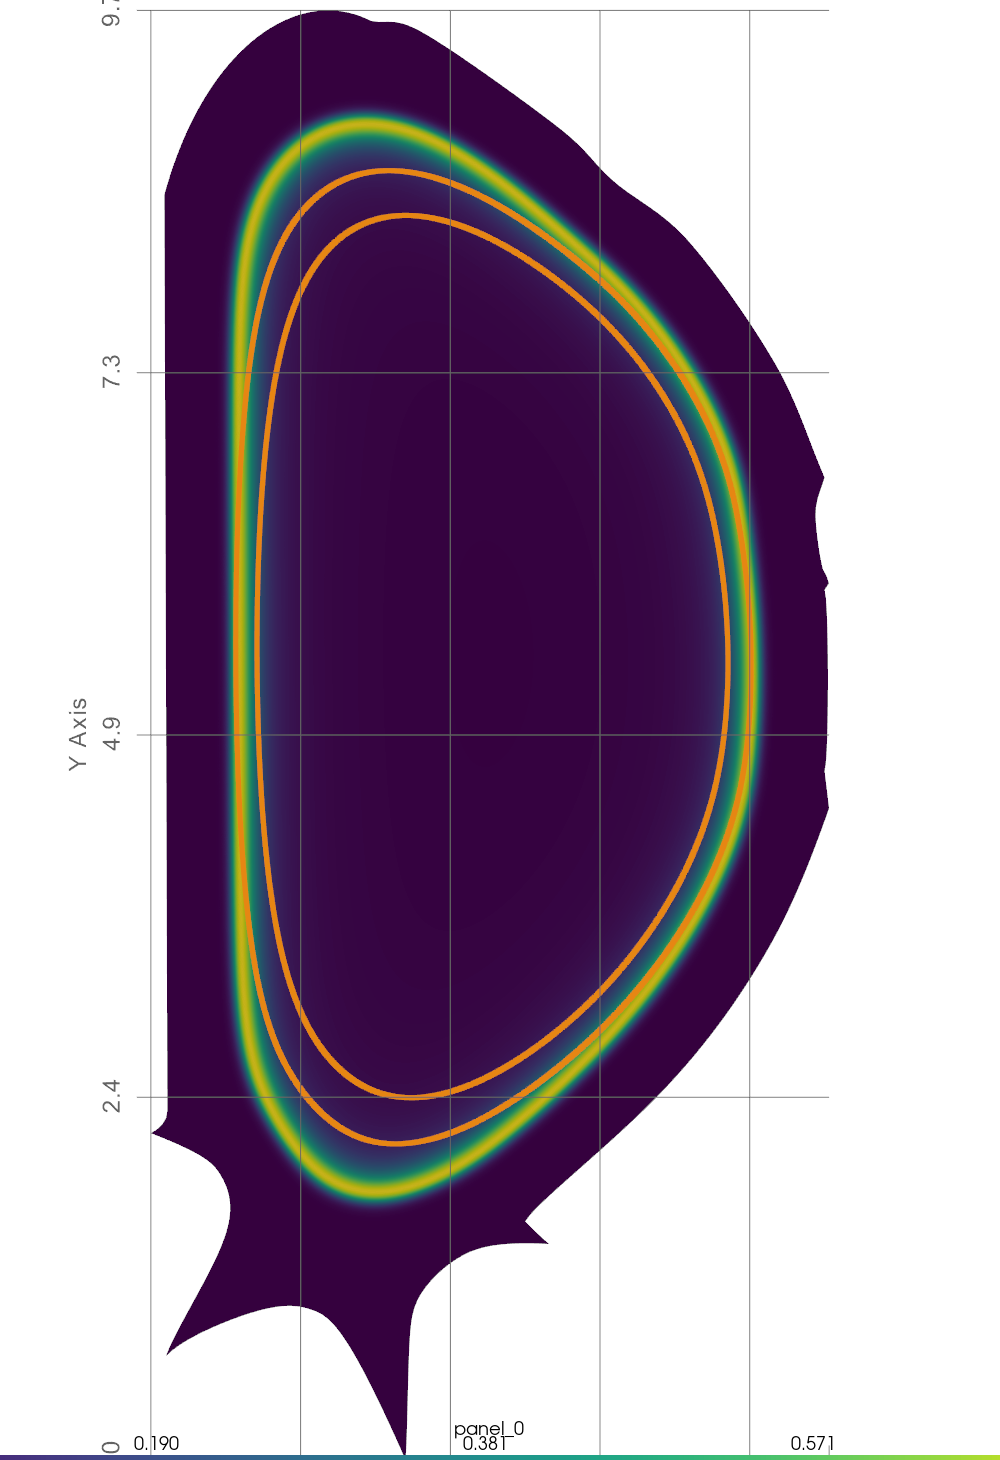
\includegraphics[width=\linewidth,height=0.35\textheight,keepaspectratio]{figures/iter_0p4_0p5_fractional_highdof_panel_03_accept_k0.png}
    \caption{First accepted state, $k=0$}
  \end{subfigure}%
  \hspace{0.01\linewidth}%
  \begin{subfigure}[t]{0.18\linewidth}
    \centering
    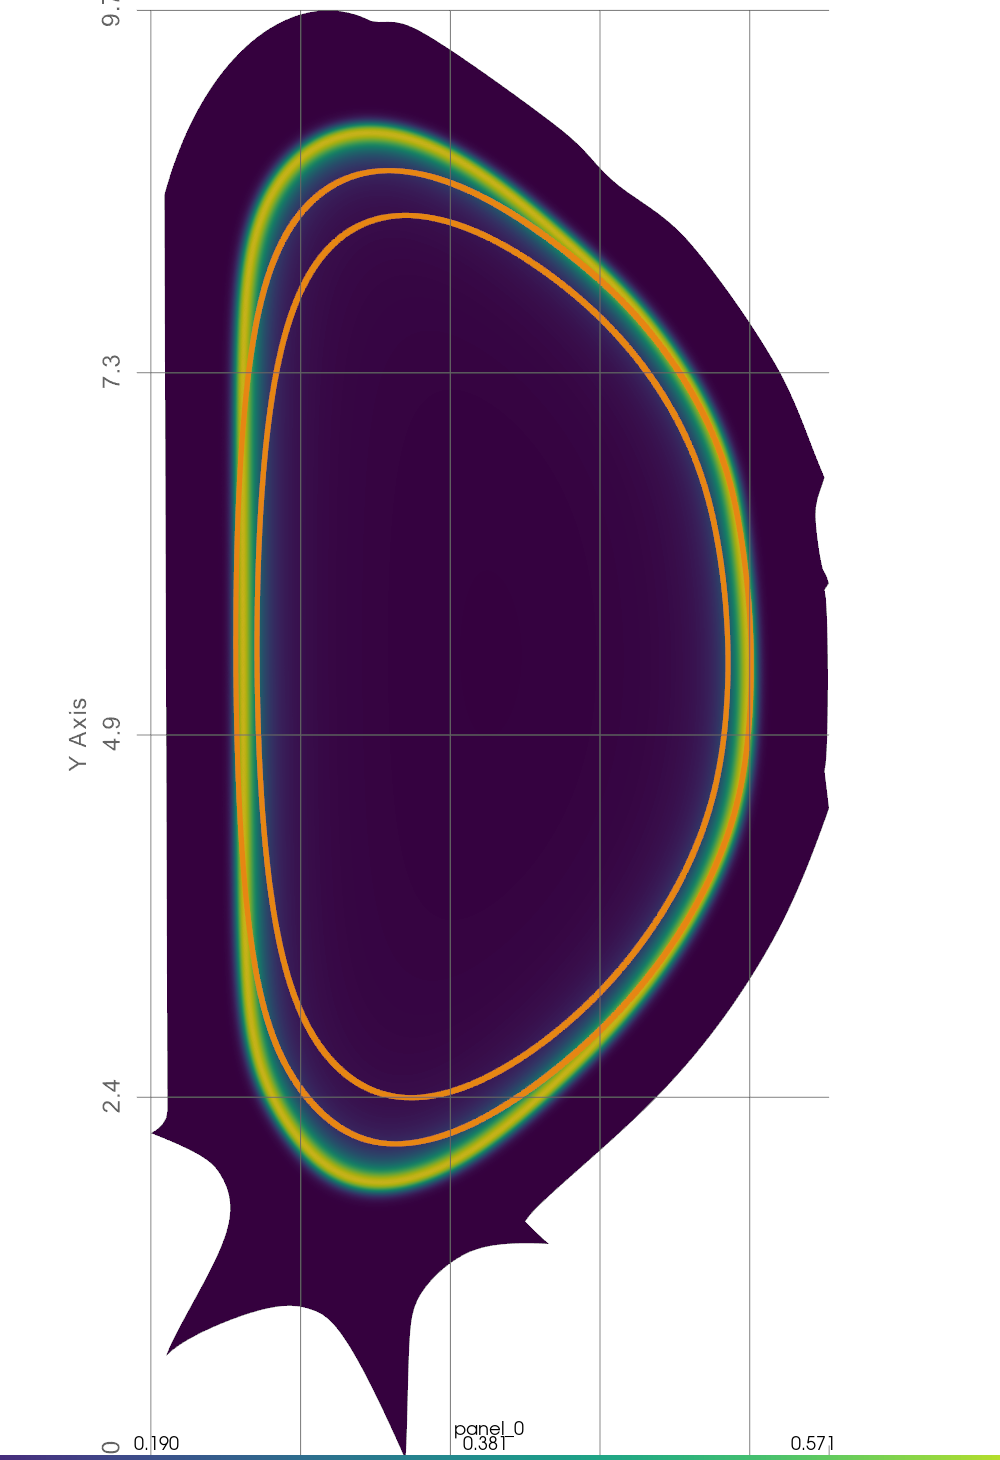
\includegraphics[width=\linewidth,height=0.35\textheight,keepaspectratio]{figures/iter_0p4_0p5_fractional_highdof_panel_04_accept_k5.png}
    \caption{Translated band, $k=5$}
  \end{subfigure}}

  \vspace{1mm}

  \makebox[\linewidth][c]{%
  \begin{subfigure}[t]{0.18\linewidth}
    \centering
    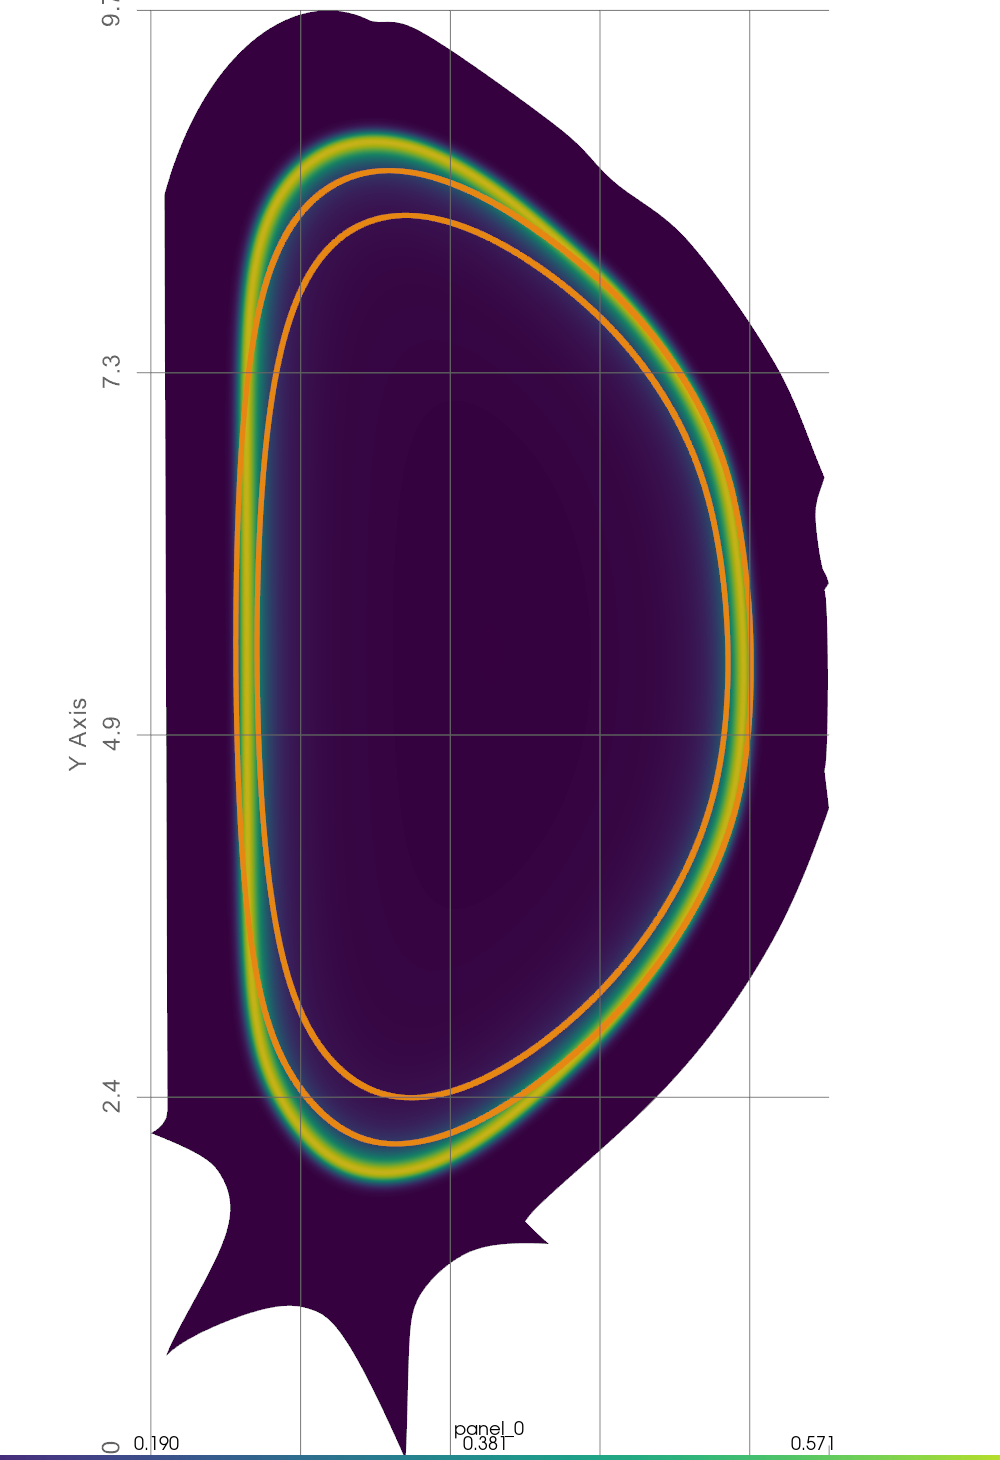
\includegraphics[width=\linewidth,height=0.35\textheight,keepaspectratio]{figures/iter_0p4_0p5_fractional_highdof_panel_05_accept_k10.png}
    \caption{Translated band, $k=10$}
  \end{subfigure}%
  \hspace{0.01\linewidth}%
  \begin{subfigure}[t]{0.18\linewidth}
    \centering
    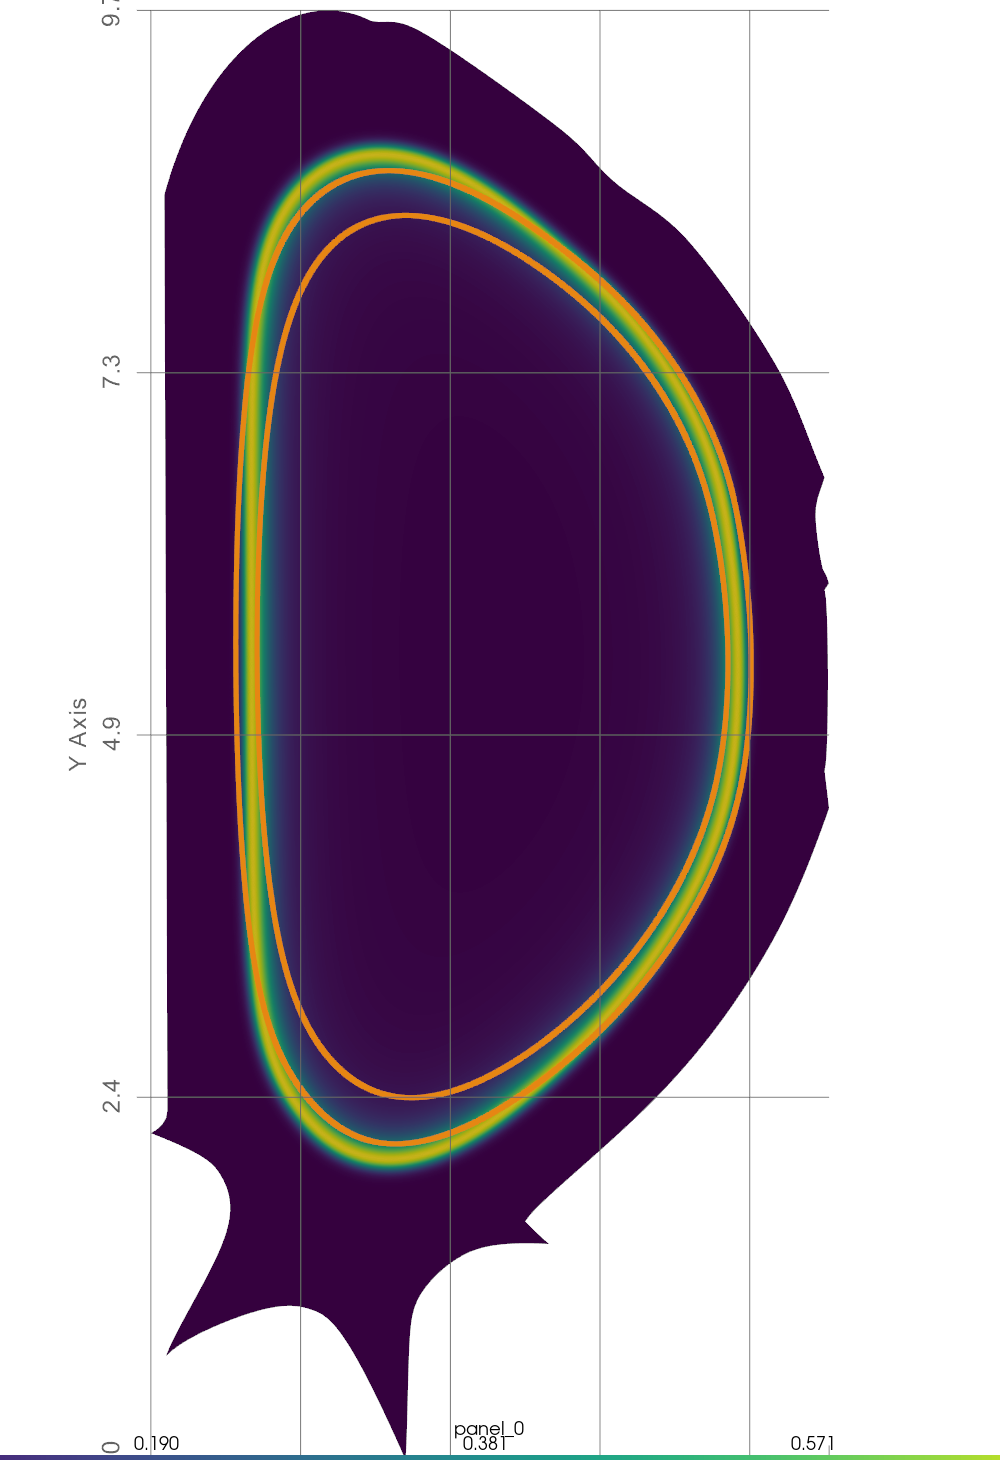
\includegraphics[width=\linewidth,height=0.35\textheight,keepaspectratio]{figures/iter_0p4_0p5_fractional_highdof_panel_06_best_k17.png}
    \caption{Best Jaccard, $k=17$}
  \end{subfigure}%
  \hspace{0.01\linewidth}%
  \begin{subfigure}[t]{0.18\linewidth}
    \centering
    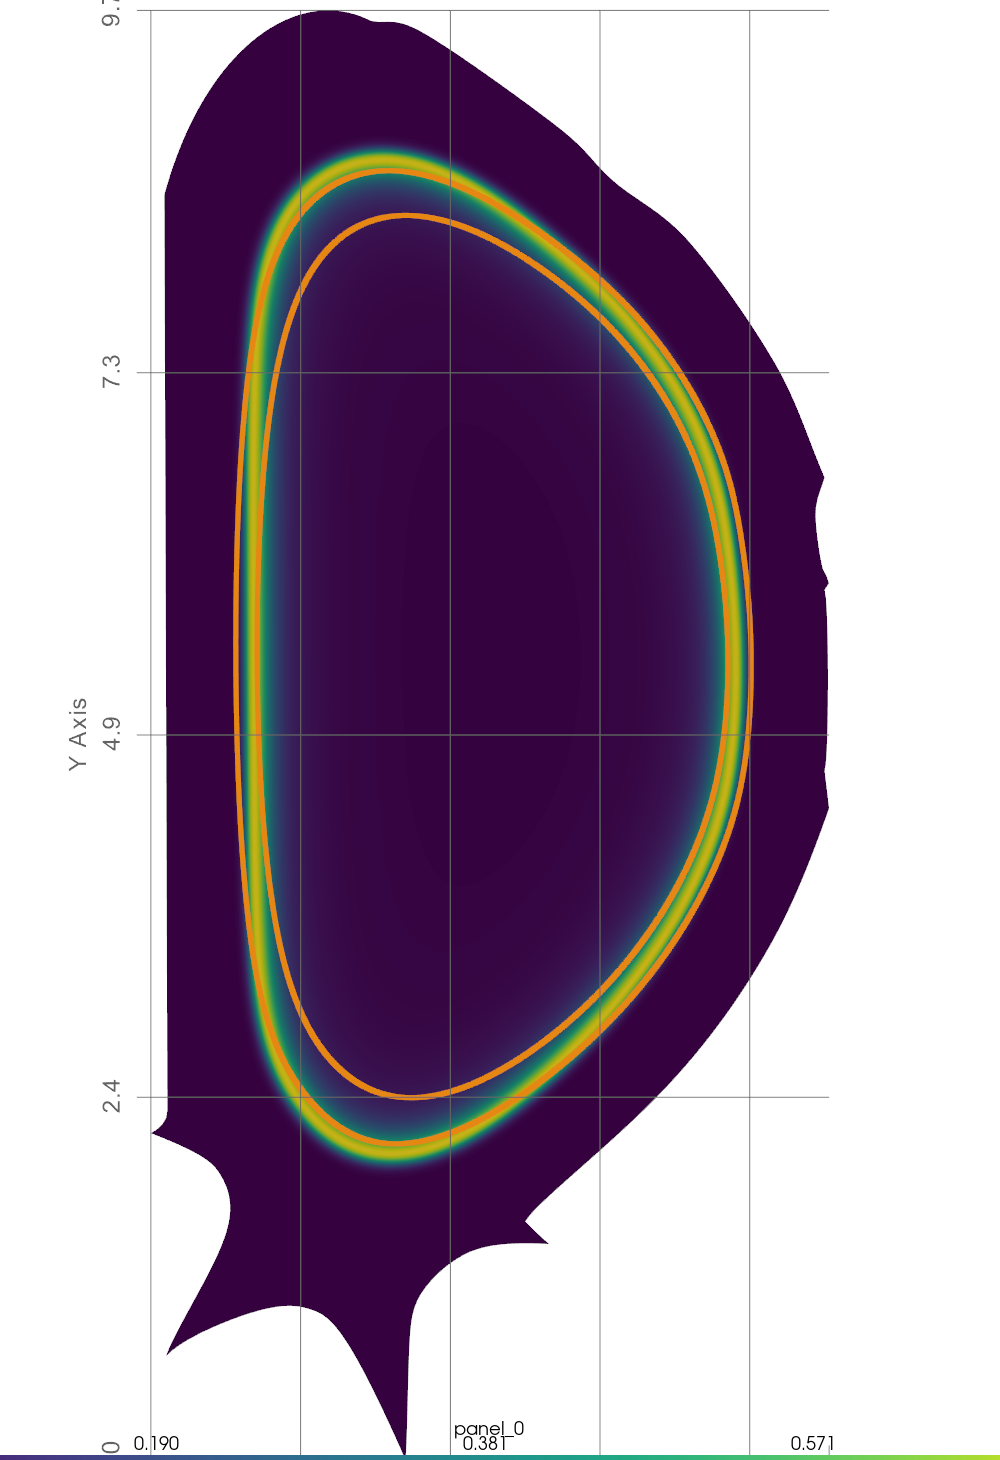
\includegraphics[width=\linewidth,height=0.35\textheight,keepaspectratio]{figures/iter_0p4_0p5_fractional_highdof_panel_07_stagnation_k20.png}
    \caption{Stagnation trigger, $k=20$}
  \end{subfigure}%
  \hspace{0.01\linewidth}%
  \begin{subfigure}[t]{0.18\linewidth}
    \centering
    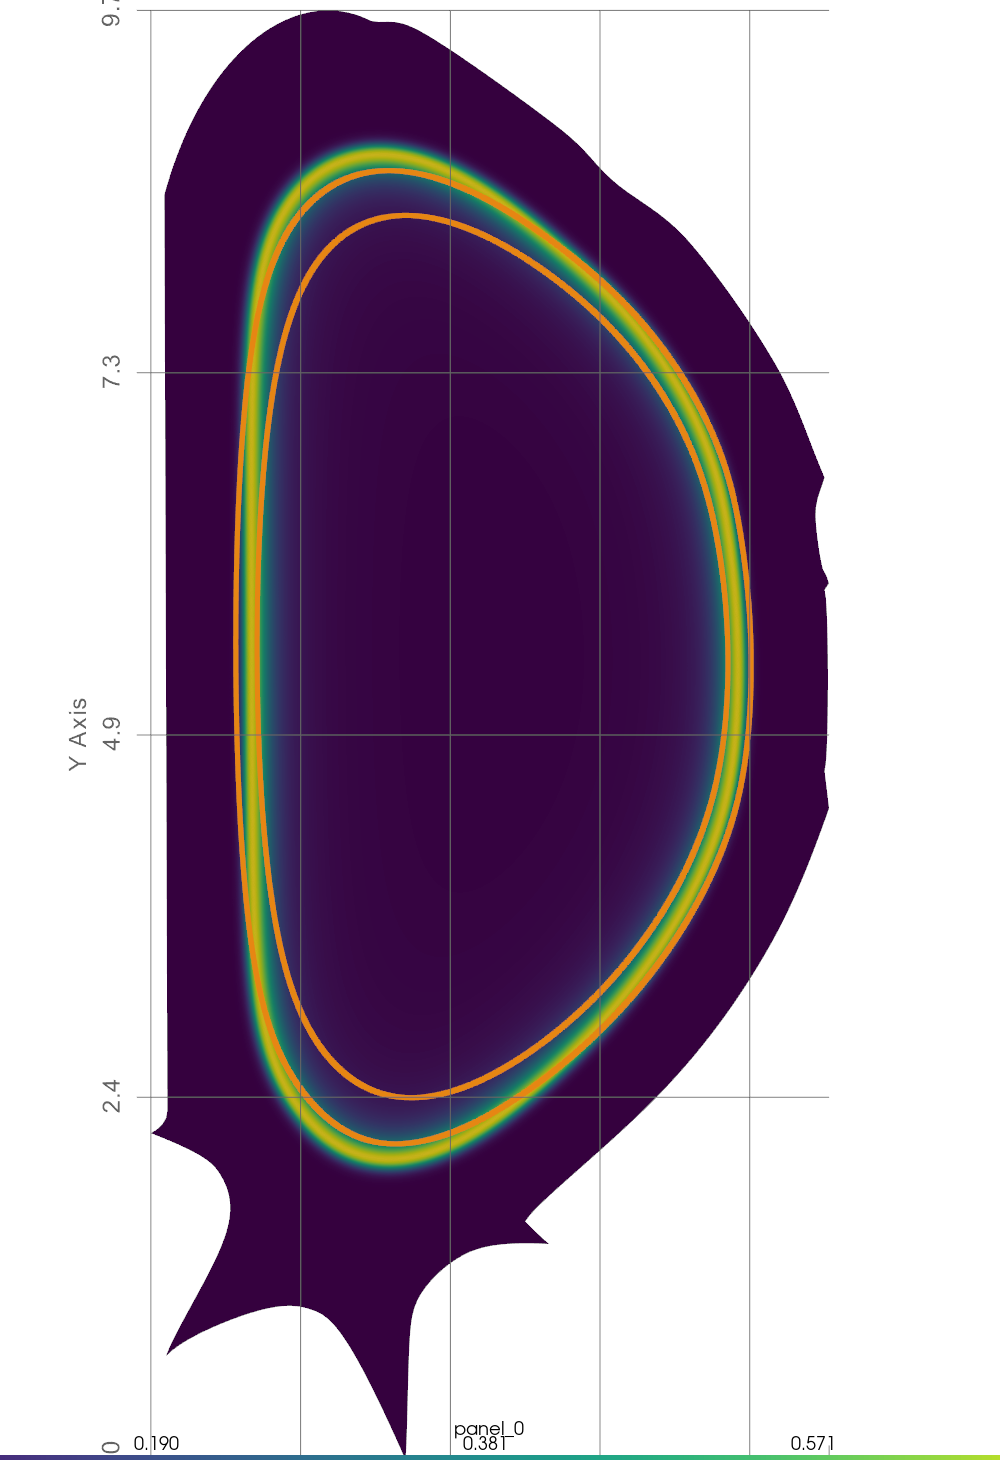
\includegraphics[width=\linewidth,height=0.35\textheight,keepaspectratio]{figures/iter_0p4_0p5_fractional_highdof_panel_08_final.png}
    \caption{Restored final state}
  \end{subfigure}}
  \caption{High-resolution evolution of the lower ITER band under direct,
  no-homotopy fractional initialization. The target density is shown once;
  the other panels show the equilibrium density with the prescribed torsion
  band retained as orange contours. The first reduced step reaches the
  minimum threshold width without leaving the relevant branch. Subsequent
  accepted states translate that band toward larger potential, after which
  the active-set overlap plateaus and the best-Jaccard state is restored.}
  \label{fig:iter-fractional-0p4-0p5-storyboard}
  \end{minipage}
\end{figure}
\end{landscape}

The first reduced trial projected the thresholds to
\[
  (c_{1,\phi},c_{2,\phi})=(0.06829502,0.08029502),
  \qquad \Delta c_\phi=0.012,
\]
where the width attained its lower bound. Unlike the minimum-width trial for
the $[0.6,0.7]T_{\max}$ band, this state remained on the relevant outer
branch. It converged in six Newton updates to
$1.368\times10^{-14}$ and was accepted, while its active Jaccard index
increased from $0.2690$ to $0.3546$. Every subsequent trial was also
accepted. The width remained fixed at $0.012$ and the optimizer translated
both thresholds upward; each of the remaining 20 trials required three
Newton updates. Across all 21 accepted trials, the terminal residual stayed
between $1.368\times10^{-14}$ and $1.427\times10^{-14}$. There were no
rejected threshold pairs, and the absolute trust radius remained
$9.671\times10^{-3}$ throughout.

\begin{figure}[p]
  \centering
  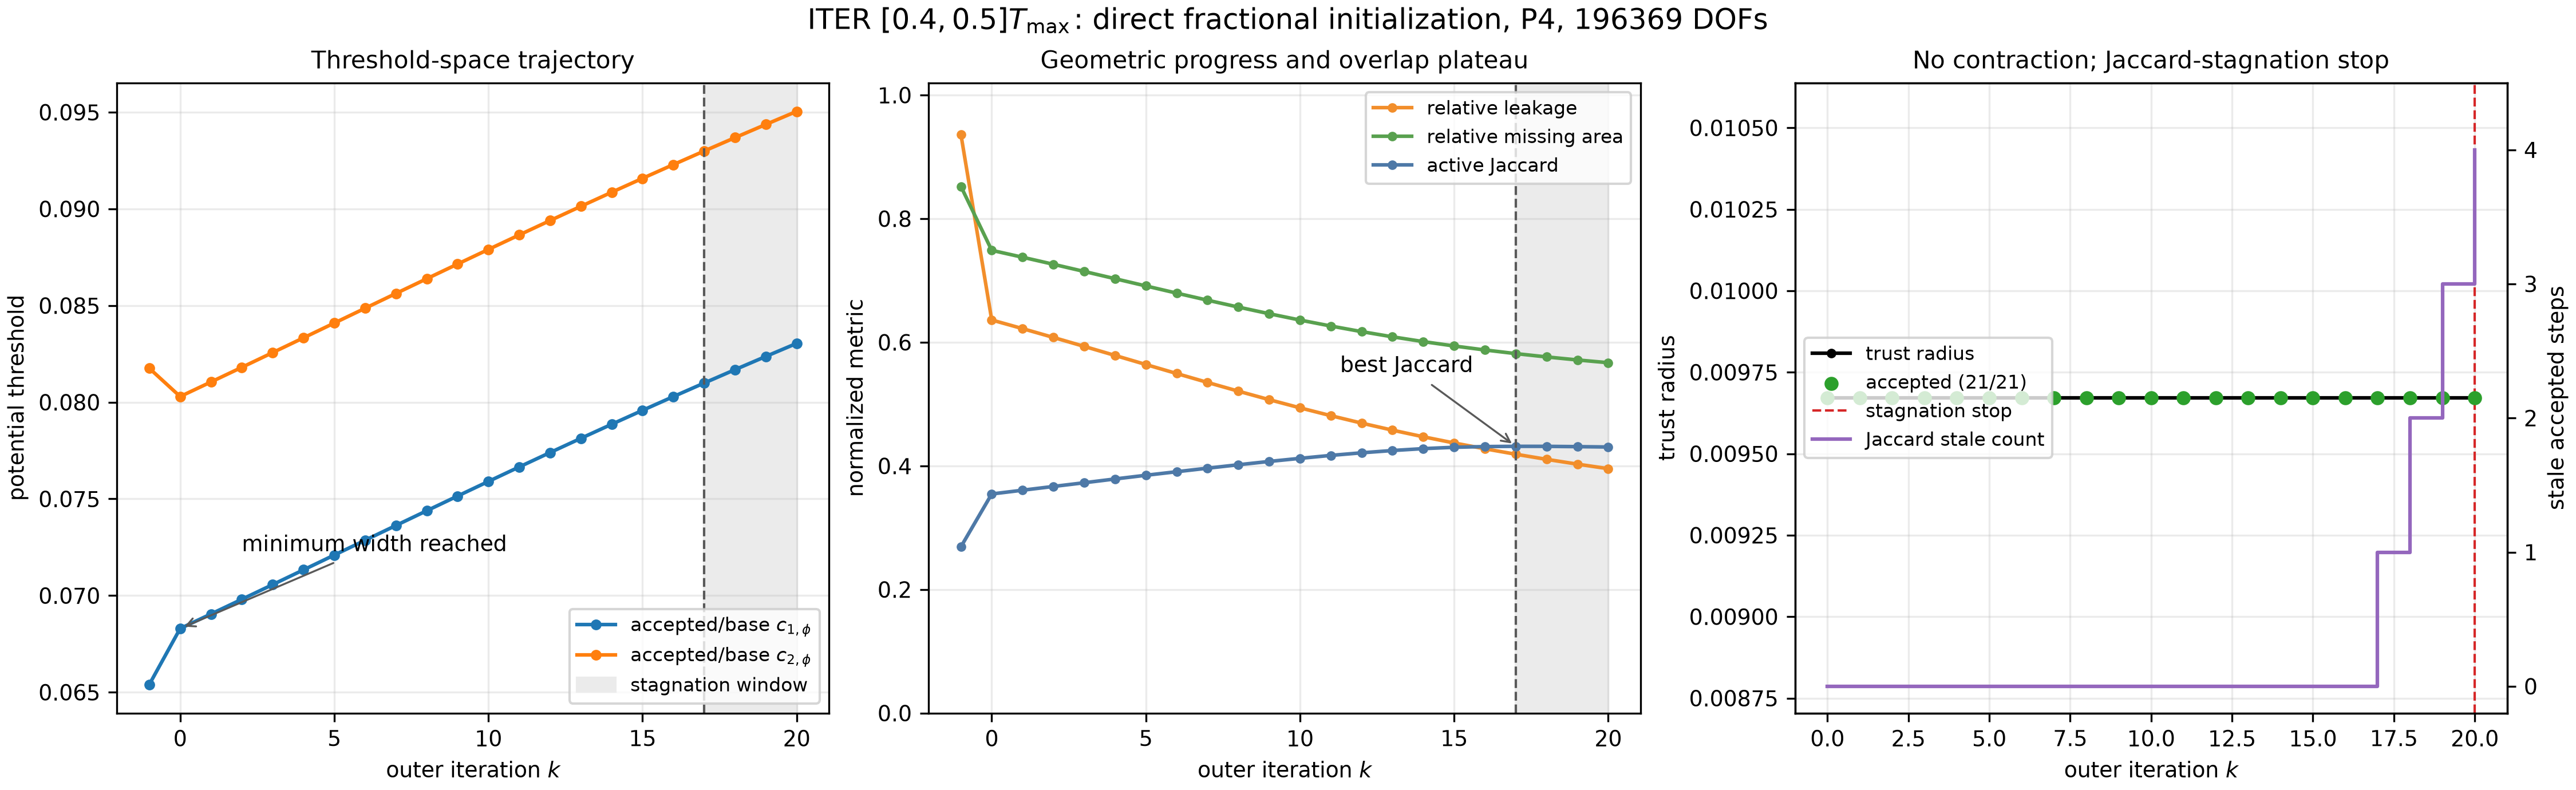
\includegraphics[width=\linewidth]{figures/iter_0p4_0p5_fractional_highdof_optimization_trace.png}
  \caption{Threshold and geometric history for the lower-band direct
  fractional-initialization run. Left: the seed first contracts to the
  minimum width, after which both thresholds translate together. Centre:
  smooth relative leakage and missing area decrease while the hard active
  Jaccard index rises to its maximum at $k=17$ and then changes by less than
  the configured stagnation tolerance. Right: all 21 trials are accepted, so
  the trust radius does not contract; the four-step Jaccard stale count
  triggers termination at $k=20$.}
  \label{fig:iter-fractional-0p4-0p5-trace}
\end{figure}

\begin{table}[htbp]
  \centering
  \caption{Selected fully converged states from the lower-band direct
  fractional-initialization experiment. $L_{\rm rel}$ and $M_{\rm rel}$
  denote relative leakage and relative missing area. The terminal
  stagnation state is followed by the best-Jaccard state restored for final
  output.}
  \label{tab:iter-fractional-0p4-0p5}
  \resizebox{\linewidth}{!}{%
  \begin{tabular}{@{}lrrrrrr@{}}
    \toprule
    state & $c_{1,\phi}$ & $c_{2,\phi}$ & residual
      & $L_{\rm rel}$ & $M_{\rm rel}$ & active Jaccard \\
    \midrule
    projected direct seed
      & 0.065403 & 0.081754 & $1.417\times10^{-14}$
      & 0.9365 & 0.8523 & 0.2690 \\
    first accepted state ($k=0$)
      & 0.068295 & 0.080295 & $1.368\times10^{-14}$
      & 0.6361 & 0.7488 & 0.3546 \\
    translated state ($k=10$)
      & 0.075903 & 0.087903 & $1.401\times10^{-14}$
      & 0.4939 & 0.6360 & 0.4122 \\
    stagnation trigger ($k=20$)
      & 0.083044 & 0.095044 & $1.420\times10^{-14}$
      & 0.3955 & 0.5670 & 0.4306 \\
    restored best-Jaccard state ($k=17$)
      & 0.080993 & 0.092993 & $1.413\times10^{-14}$
      & 0.4189 & 0.5817 & 0.4317 \\
    \bottomrule
  \end{tabular}%
  }
\end{table}

The accepted active-Jaccard history increased monotonically from $0.2690$ at
the seed to $0.4317$ at $k=17$, then took the values
$0.4316$, $0.4311$, and $0.4306$. The four-step stale counter therefore
terminated the threshold loop with
\texttt{CONVERGED\_JACCARD\_STAGNATION} at $k=20$. The projected-gradient
norm was still $2.41\times10^2$, so this label denotes the configured
active-set-overlap plateau rather than first-order stationarity. Restoration
returned the thresholds to the best observed Jaccard pair at $k=17$. Its
residual already satisfied the final tolerance, and the final exact Newton
call required zero updates.

The restoration criterion explains an apparent reversal in
Table~\ref{tab:iter-fractional-0p4-0p5}: the smooth leakage and missing-area
measures continued to decrease through $k=20$, but the hard active Jaccard
index had already begun to fall. At the restored state, active recall was
$0.9949$, active precision was $0.4326$, and the Dice coefficient was
$0.6030$. The active area was $2.5315$ versus target area $3.0239$, or
$83.72\%$ of the target.

The certified core nevertheless had zero area. At the enforced minimum width,
$\Delta c_\phi=0.012=4\varepsilon_\phi$; with $\kappa=2$, the certified
interval
$[c_{1,\phi}+2\varepsilon_\phi,c_{2,\phi}-2\varepsilon_\phi]$ collapses to a
single level. Thus this is a successful direct nonlinear initialization and
a complete, deliberately terminated reduced-optimization run, but not
certified-subband geometric convergence. It is notably more robust than the
corresponding $[0.6,0.7]T_{\max}$ experiment: it required no homotopy, no
rejected trial, and no trust-radius contraction. The noninteractive run took
$218.86\,\mathrm{s}$; an otherwise equivalent plotting run took
$254.68\,\mathrm{s}$ and reproduced the reported thresholds and metrics to
roundoff.
\clearpage
\subsection{No-homotopy direct fractional initialization for the near-boundary ITER band}
\label{sec:iter-fractional-0p1-0p2}
We repeated the direct fractional-initialization experiment for the
near-boundary ITER torsion band
$0.1\,T_{\max}\leq T\leq0.2\,T_{\max}$ with the script
\begin{center}
  \small
  \texttt{scripts/diocotron\_dolfinx/}\\[-0.2ex]
  \texttt{dolfinx\_torsion\_fractional\_phi\_target\_window\_}\\[-0.2ex]
  \texttt{reduced\_optimization.py}
\end{center}
As in Section~\ref{sec:iter-fractional-0p4-0p5}, the run used neither an
$L^2$/quantile fit nor an $H^{-1}$ threshold search, and it was not supplied
with a previous equilibrium. The target potential had
$\|\phi_T\|_{L^\infty}=0.07742247$, giving the raw fractional pair
\[
  (c_{1,\phi}^{\rm raw},c_{2,\phi}^{\rm raw})
  =(0.1,0.2)\,\|\phi_T\|_{L^\infty}
  =(0.00774225,0.01548449).
\]
Its width, $0.00774225$, was below the admissible minimum $0.012$. The
threshold projection therefore widened the pair symmetrically about its
midpoint before the nonlinear solve:
\[
  (c_{1,\phi}^{(0)},c_{2,\phi}^{(0)})
  =(0.00561337,0.01761337),
  \qquad \Delta c_\phi^{(0)}=0.012.
\]
For this saved execution the projected direct Newton solve succeeded, so no
source homotopy was used. In particular, the recorded initialization contains
only direct Newton states and no homotopy stage.

The discretization and nonlinear accuracy matched the preceding
high-resolution ITER tests: 24,430 triangular cells, a P4 space with 196,369
global degrees of freedom, quadrature degree 16, a sharp target indicator
($\varepsilon_T=0$), and fixed equilibrium smoothing
$\varepsilon_\phi=0.003$. Eight MPI ranks, one numerical-library thread per
rank, and MUMPS were used. Initial, trial, and final states were required to
satisfy the residual tolerance $10^{-12}$.

The projected direct seed converged without continuation. Its fifteen saved
Newton updates had the residual history
\[
\begin{aligned}
  2.240\!\times\!10^{-2}&\to1.603\!\times\!10^{-2}
  \to9.784\!\times\!10^{-3}\to9.089\!\times\!10^{-3}\\
  &\to8.604\!\times\!10^{-3}\to8.543\!\times\!10^{-3}
  \to8.303\!\times\!10^{-3}\to8.271\!\times\!10^{-3}\\
  &\to7.360\!\times\!10^{-3}\to6.337\!\times\!10^{-3}
  \to2.840\!\times\!10^{-3}\to2.722\!\times\!10^{-4}\\
  &\to7.568\!\times\!10^{-7}\to3.681\!\times\!10^{-11}
  \to5.589\!\times\!10^{-15}.
\end{aligned}
\]
Thus the reduced derivatives were first evaluated on a fully resolved
nonlinear state. The projected seed had relative leakage $0.7777$, relative
missing area $0.7218$, and active Jaccard index $0.3600$.

\begin{landscape}
\begin{figure}[p]
  \centering
  \begin{minipage}{\linewidth}
  \centering
  \captionsetup{width=\linewidth}
  \captionsetup[subfigure]{font=scriptsize,skip=1pt}
  \makebox[\linewidth][c]{%
  \begin{subfigure}[t]{0.18\linewidth}
    \centering
    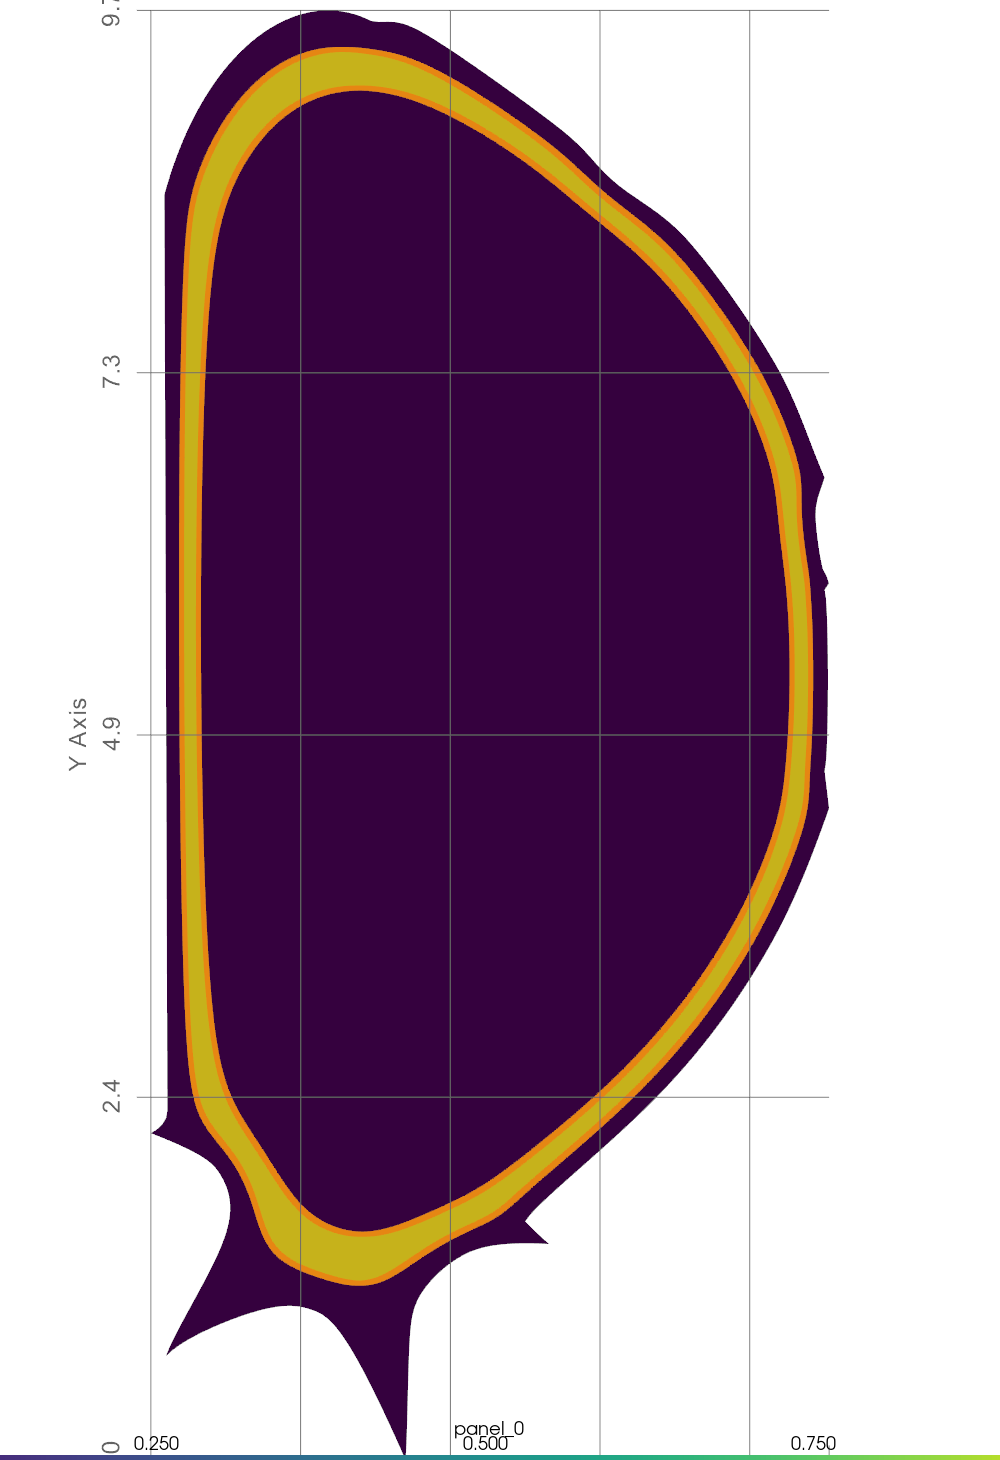
\includegraphics[width=\linewidth,height=0.35\textheight,keepaspectratio]{figures/iter_0p1_0p2_fractional_highdof_panel_01_target.png}
    \caption{Target design}
  \end{subfigure}%
  \hspace{0.01\linewidth}%
  \begin{subfigure}[t]{0.18\linewidth}
    \centering
    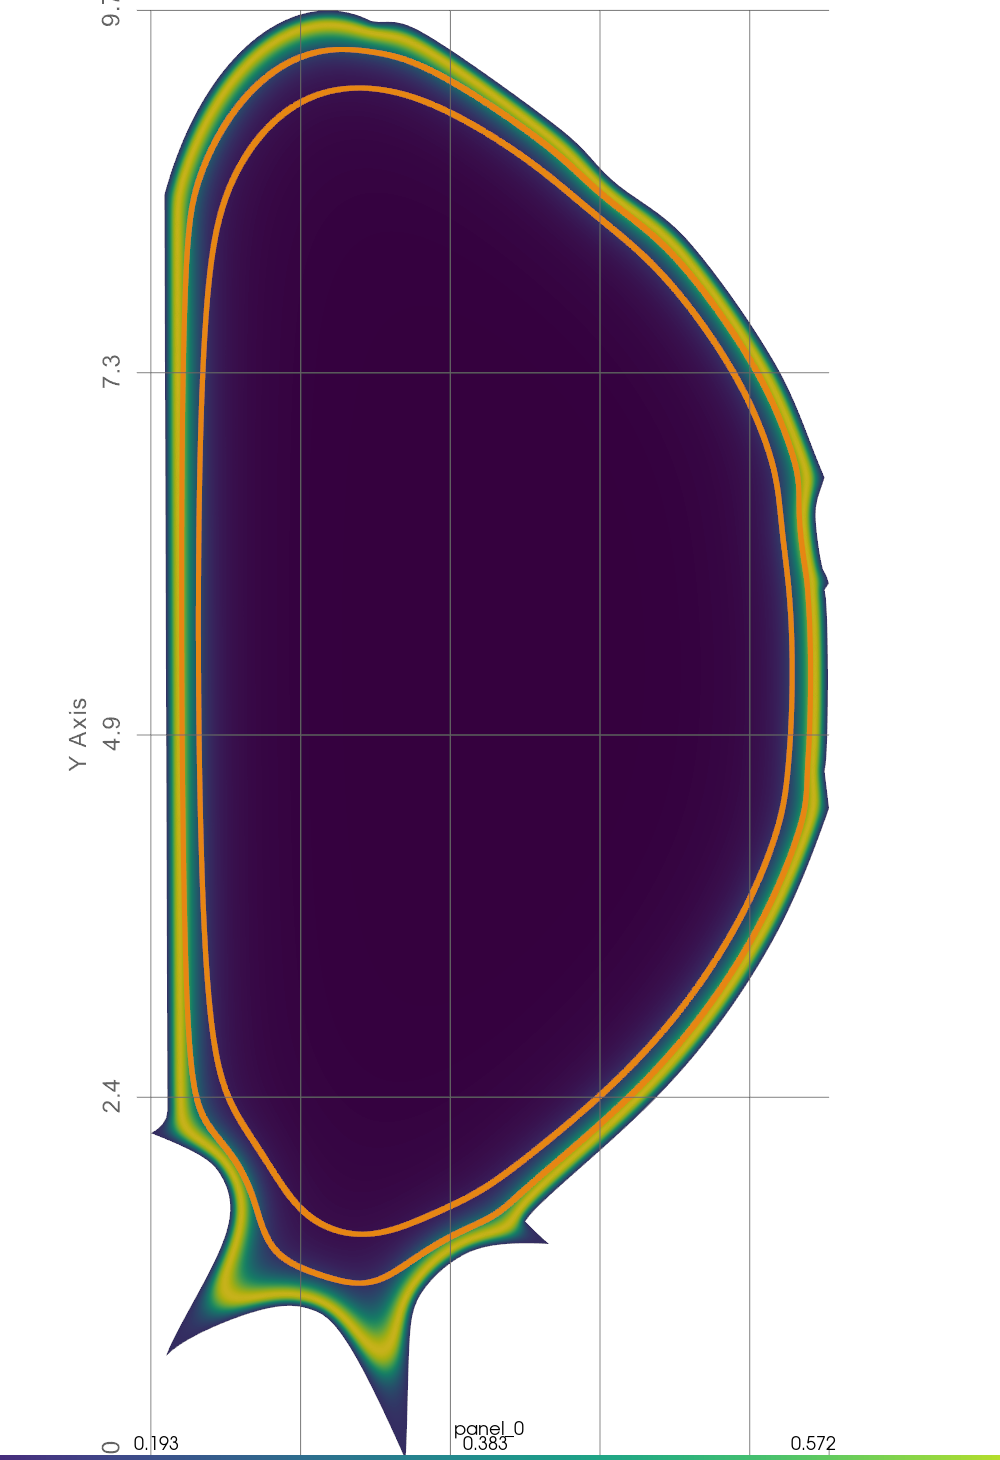
\includegraphics[width=\linewidth,height=0.35\textheight,keepaspectratio]{figures/iter_0p1_0p2_fractional_highdof_panel_02_seed.png}
    \caption{Projected direct seed}
  \end{subfigure}%
  \hspace{0.01\linewidth}%
  \begin{subfigure}[t]{0.18\linewidth}
    \centering
    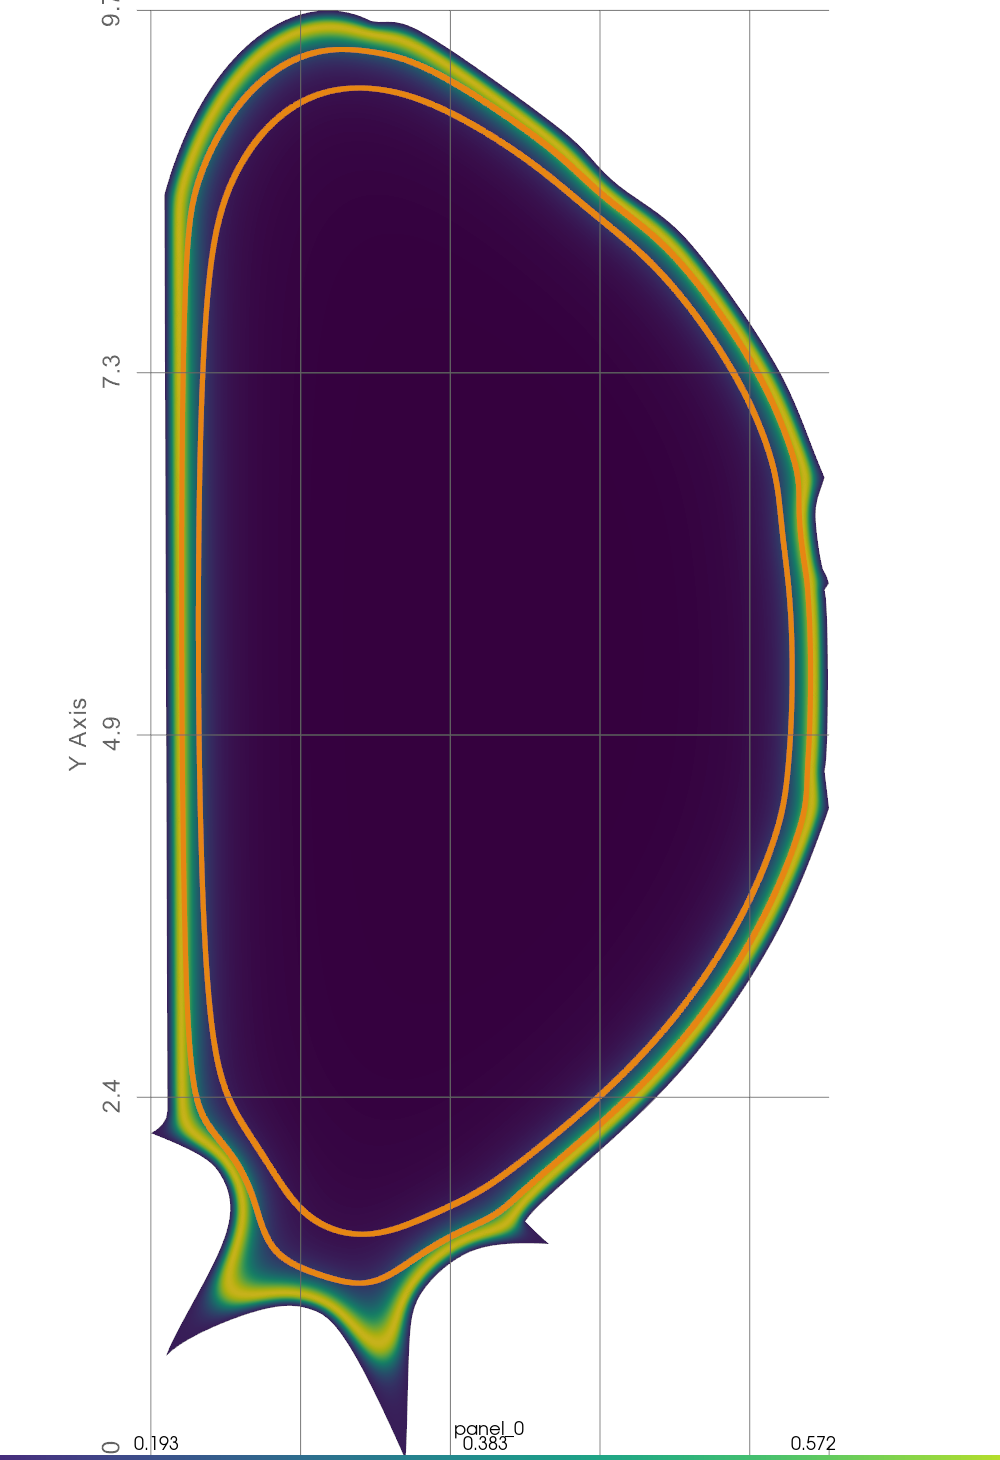
\includegraphics[width=\linewidth,height=0.35\textheight,keepaspectratio]{figures/iter_0p1_0p2_fractional_highdof_panel_03_accept_k0.png}
    \caption{First accepted state, $k=0$}
  \end{subfigure}%
  \hspace{0.01\linewidth}%
  \begin{subfigure}[t]{0.18\linewidth}
    \centering
    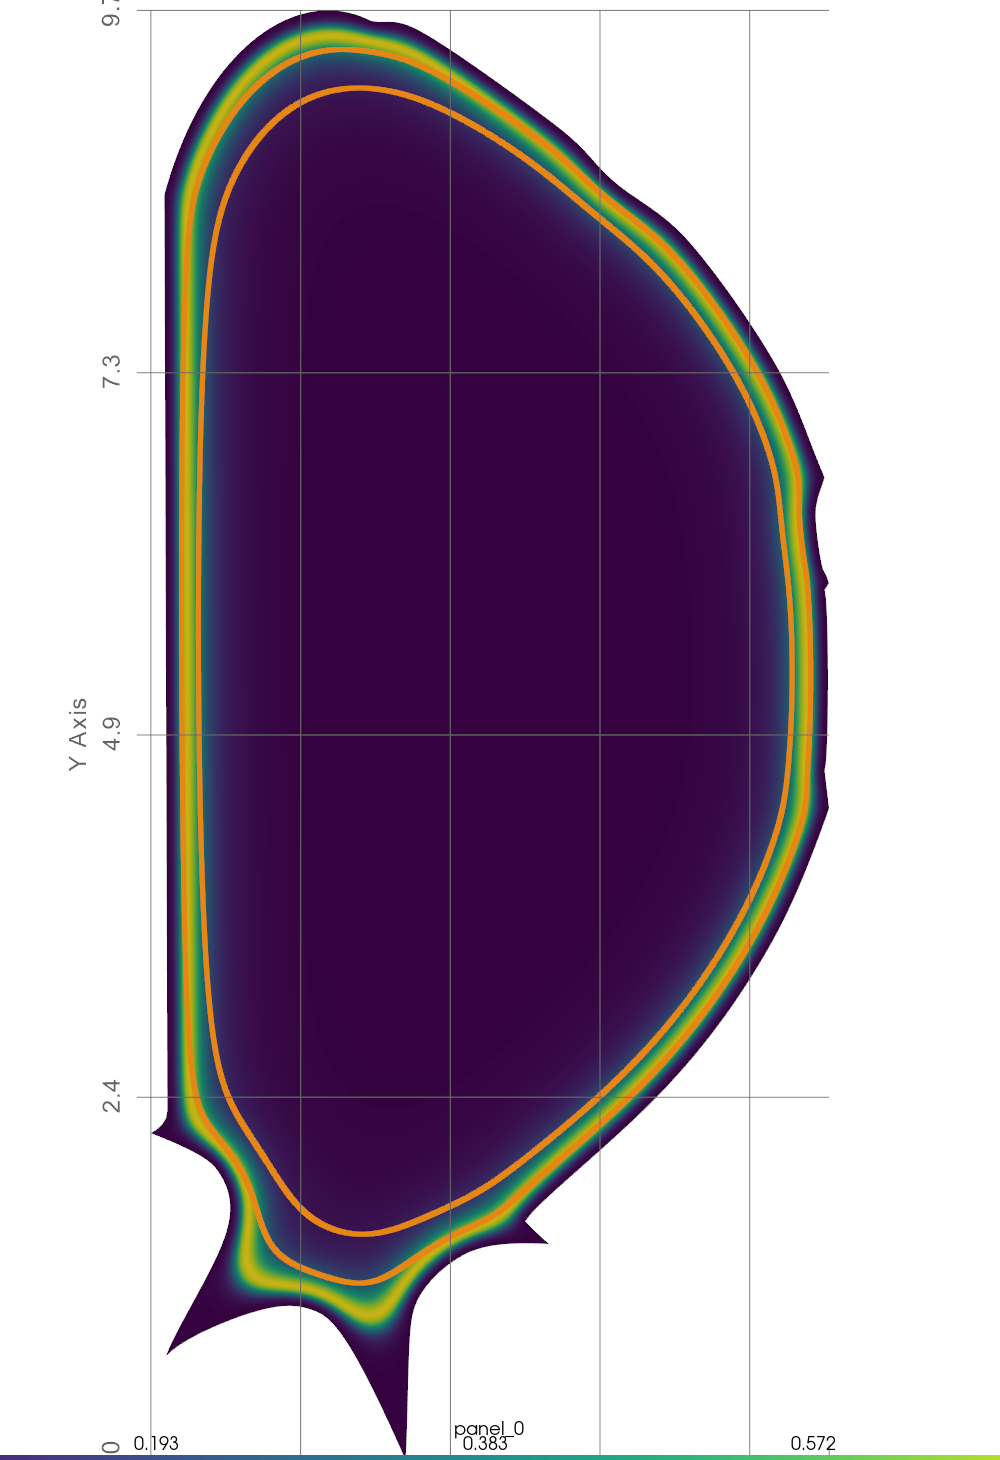
\includegraphics[width=\linewidth,height=0.35\textheight,keepaspectratio]{figures/iter_0p1_0p2_fractional_highdof_panel_04_accept_k4.png}
    \caption{Translated band, $k=4$}
  \end{subfigure}}

  \vspace{1mm}

  \makebox[\linewidth][c]{%
  \begin{subfigure}[t]{0.18\linewidth}
    \centering
    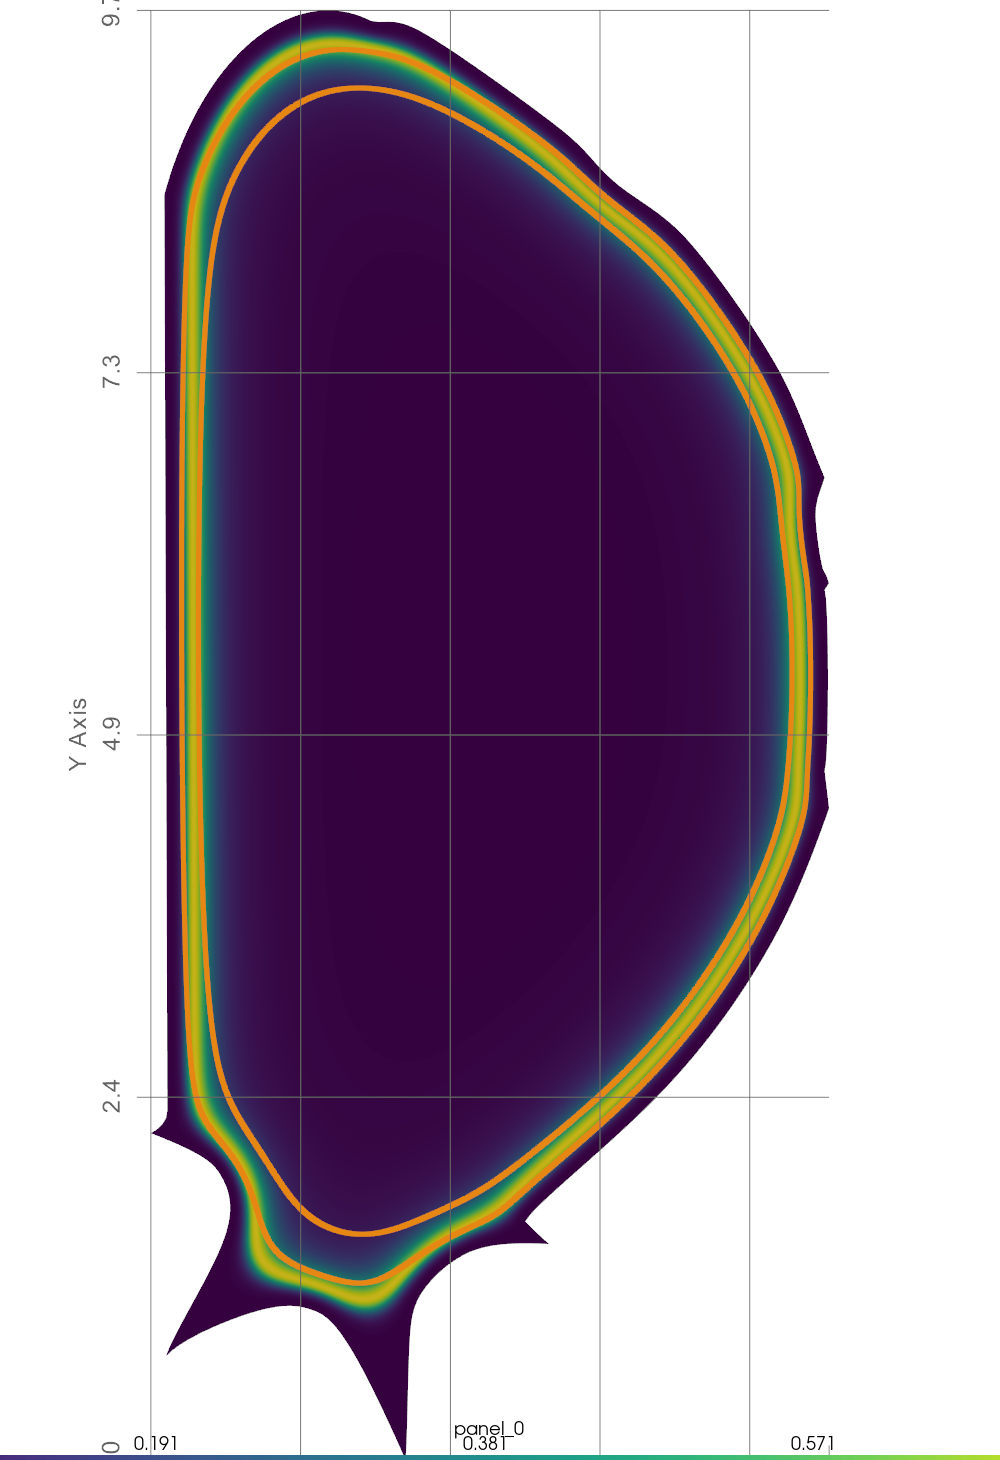
\includegraphics[width=\linewidth,height=0.35\textheight,keepaspectratio]{figures/iter_0p1_0p2_fractional_highdof_panel_05_accept_k8.png}
    \caption{Translated band, $k=8$}
  \end{subfigure}%
  \hspace{0.01\linewidth}%
  \begin{subfigure}[t]{0.18\linewidth}
    \centering
    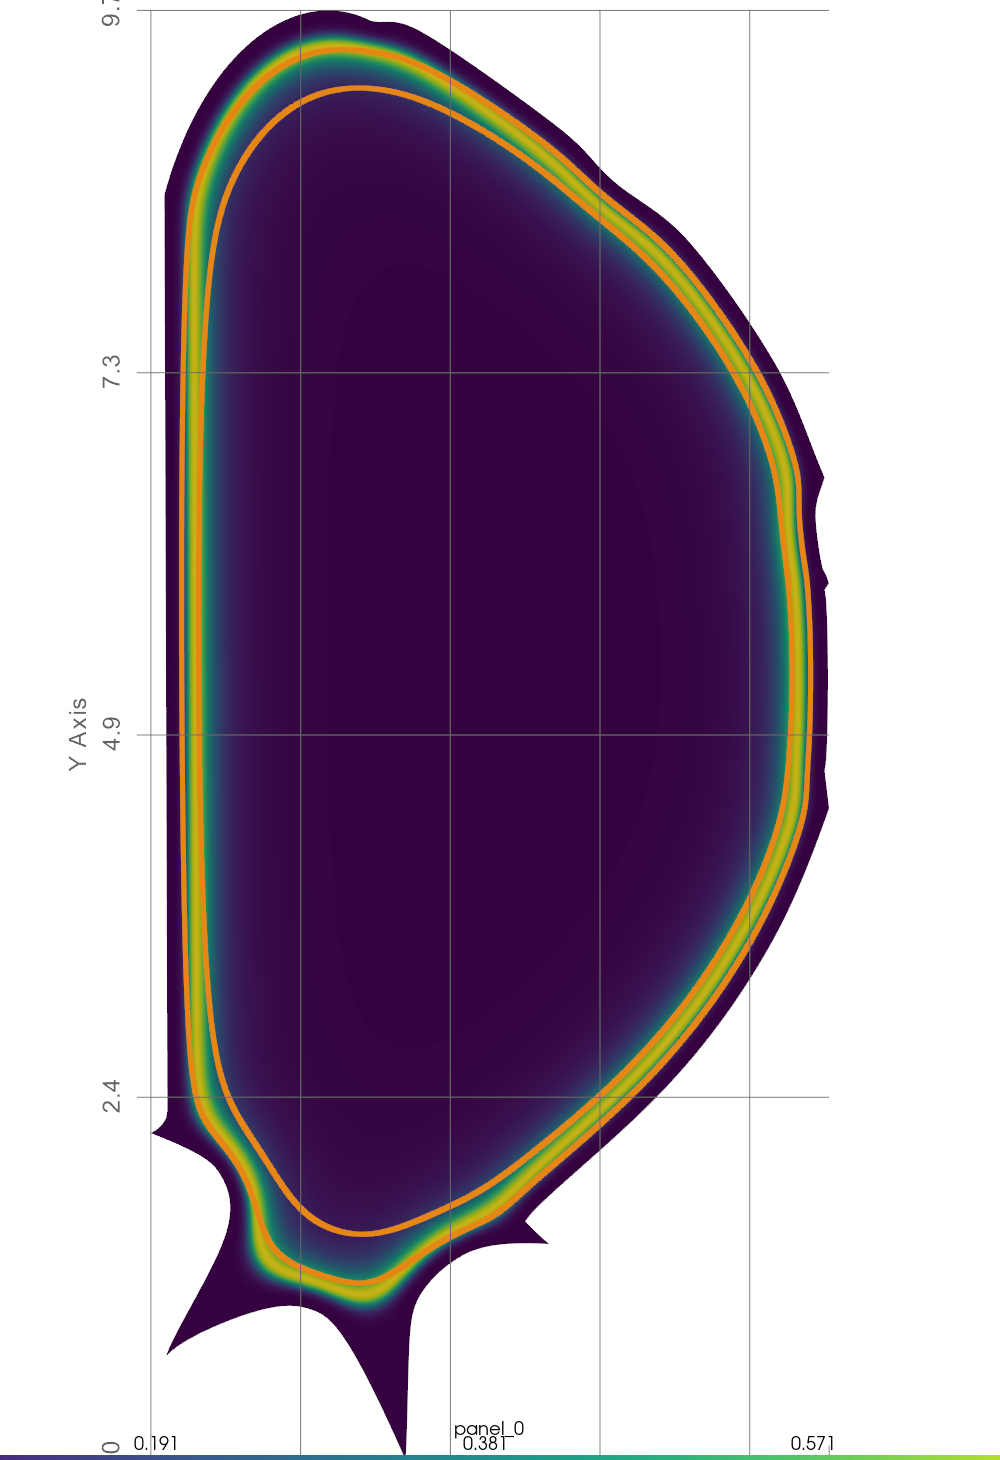
\includegraphics[width=\linewidth,height=0.35\textheight,keepaspectratio]{figures/iter_0p1_0p2_fractional_highdof_panel_06_stale_k11.png}
    \caption{Stale window begins, $k=11$}
  \end{subfigure}%
  \hspace{0.01\linewidth}%
  \begin{subfigure}[t]{0.18\linewidth}
    \centering
    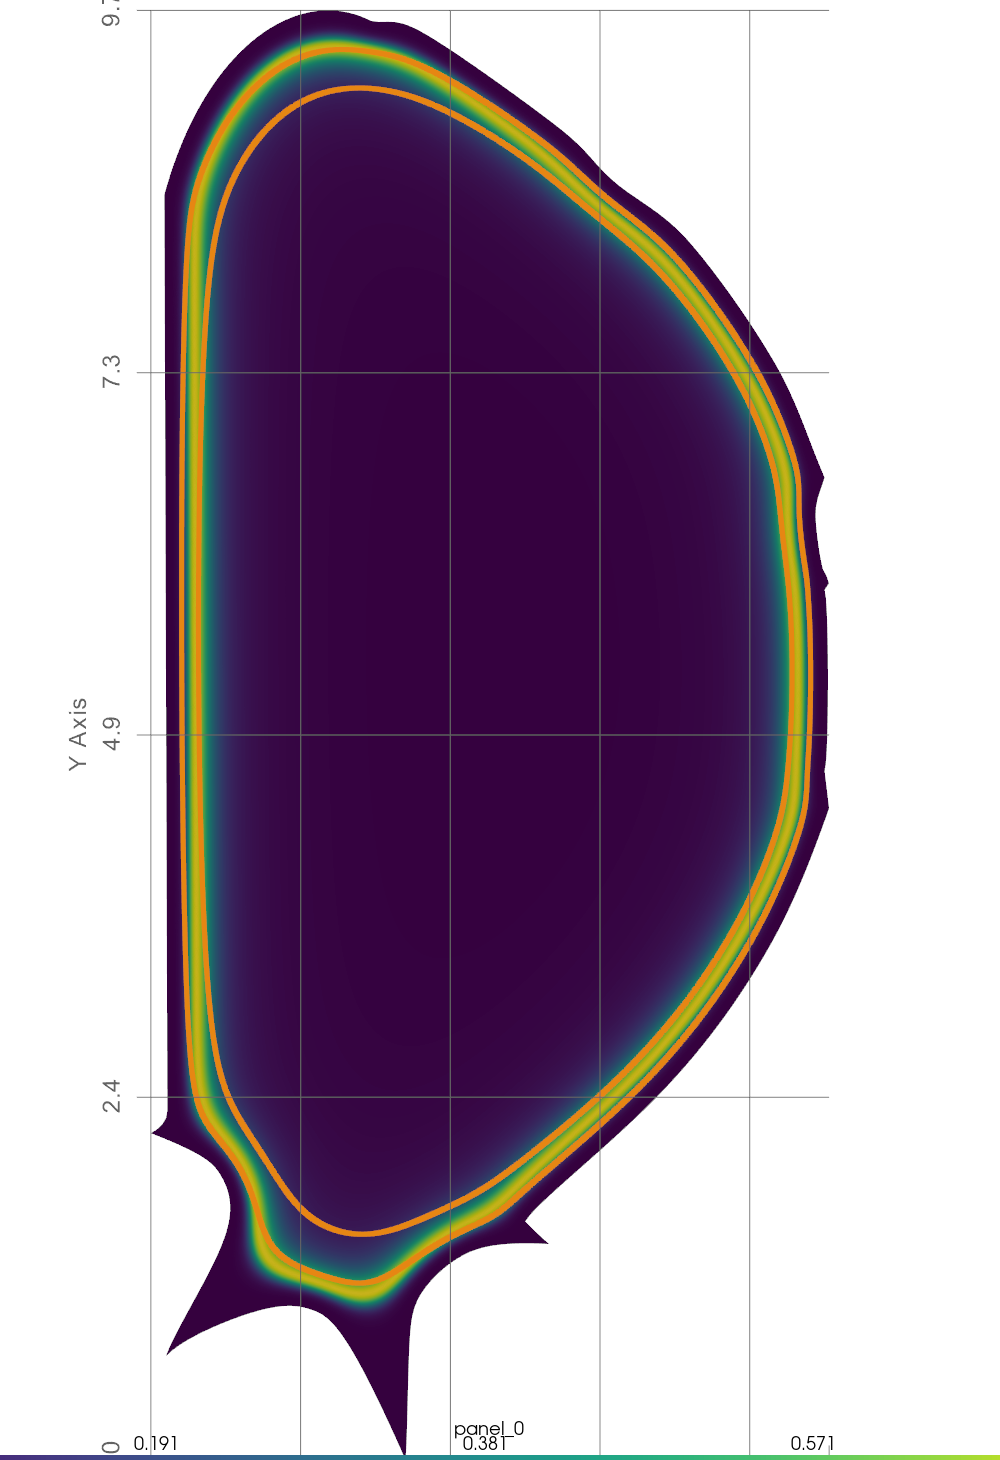
\includegraphics[width=\linewidth,height=0.35\textheight,keepaspectratio]{figures/iter_0p1_0p2_fractional_highdof_panel_07_best_stagnation_k14.png}
    \caption{Best and stop, $k=14$}
  \end{subfigure}%
  \hspace{0.01\linewidth}%
  \begin{subfigure}[t]{0.18\linewidth}
    \centering
    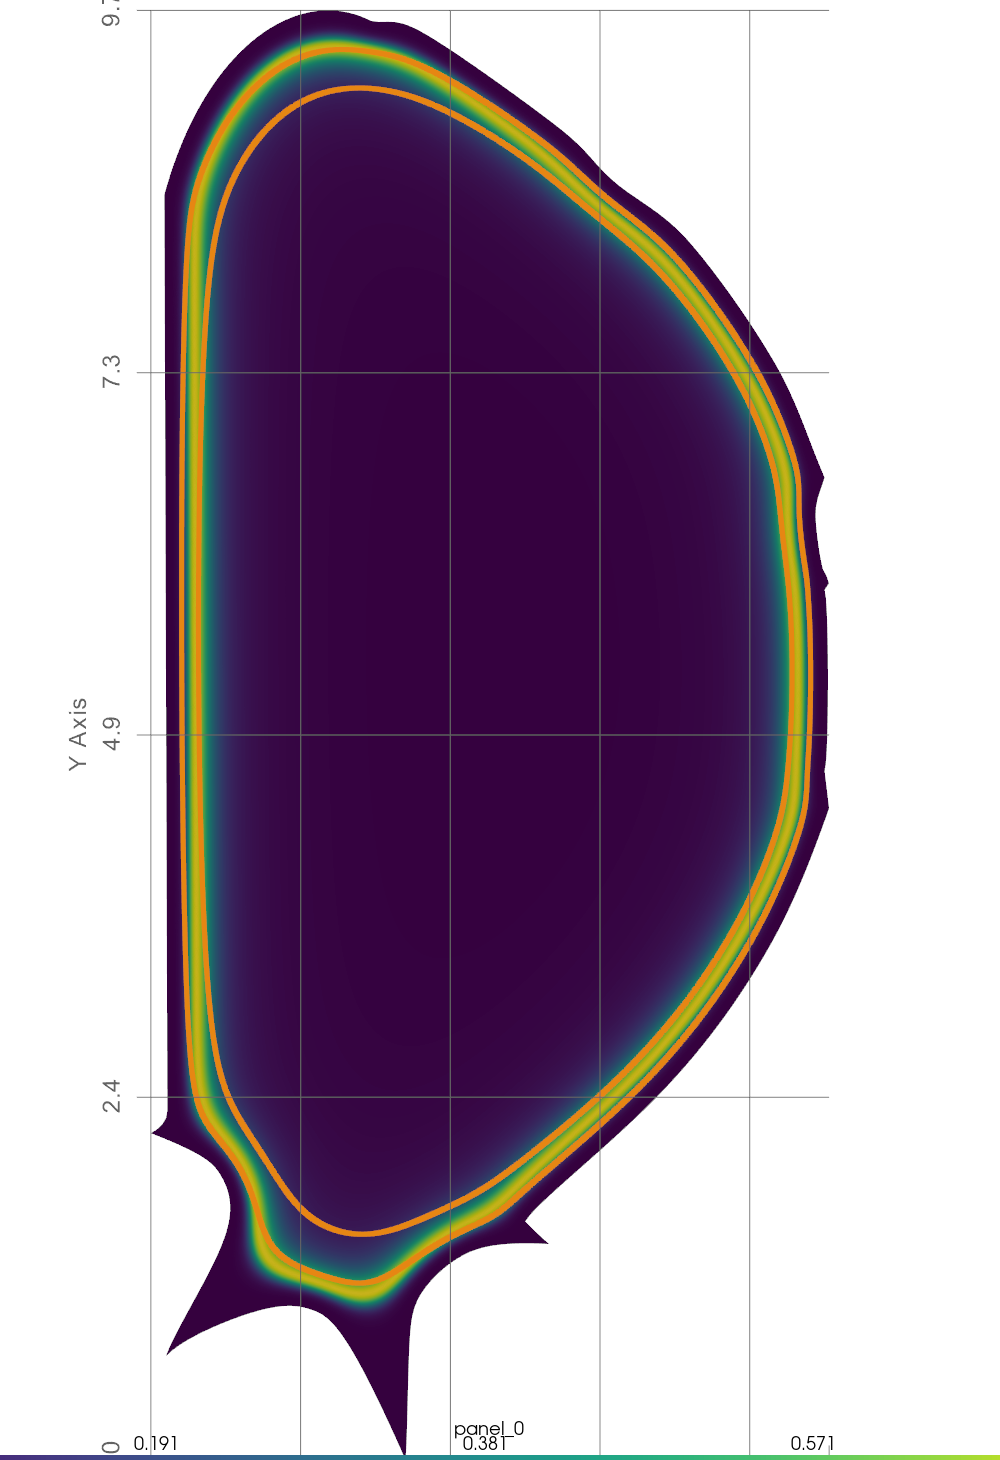
\includegraphics[width=\linewidth,height=0.35\textheight,keepaspectratio]{figures/iter_0p1_0p2_fractional_highdof_panel_08_final.png}
    \caption{Final state (unchanged)}
  \end{subfigure}}
  \caption{High-resolution evolution of the near-boundary ITER band under
  direct, no-homotopy fractional initialization. The target density is shown
  once; the other panels show the equilibrium density with the prescribed
  torsion band retained as orange contours. The raw fractional pair is first
  expanded to the minimum admissible width. The accepted states then translate
  this band toward larger potential: active overlap initially decreases,
  recovers gradually, and finally enters the configured stagnation window.
  The stopping state is also the exact best-Jaccard state, so final restoration
  leaves it unchanged.}
  \label{fig:iter-fractional-0p1-0p2-storyboard}
  \end{minipage}
\end{figure}
\end{landscape}

The projected seed already lay on the lower width bound. The first reduced
trial translated it to
\[
  (c_{1,\phi},c_{2,\phi})=(0.00709751,0.01909751),
  \qquad \Delta c_\phi=0.012.
\]
It converged in three Newton updates to $5.994\times10^{-15}$ and was
accepted, although its active Jaccard index decreased from $0.3600$ to
$0.3545$. The next accepted state reached $0.3485$; the overlap then
recovered as both thresholds continued upward. Every trial was accepted.
The first nine trials, $k=0,\ldots,8$, required three Newton updates each,
the next five required two, and the final trial required one. Across all 15
accepted trials, the terminal residual stayed between
$5.994\times10^{-15}$ and $9.423\times10^{-13}$. There were no rejected
threshold pairs, and the absolute trust radius remained
$9.671\times10^{-3}$ throughout.

\begin{figure}[p]
  \centering
  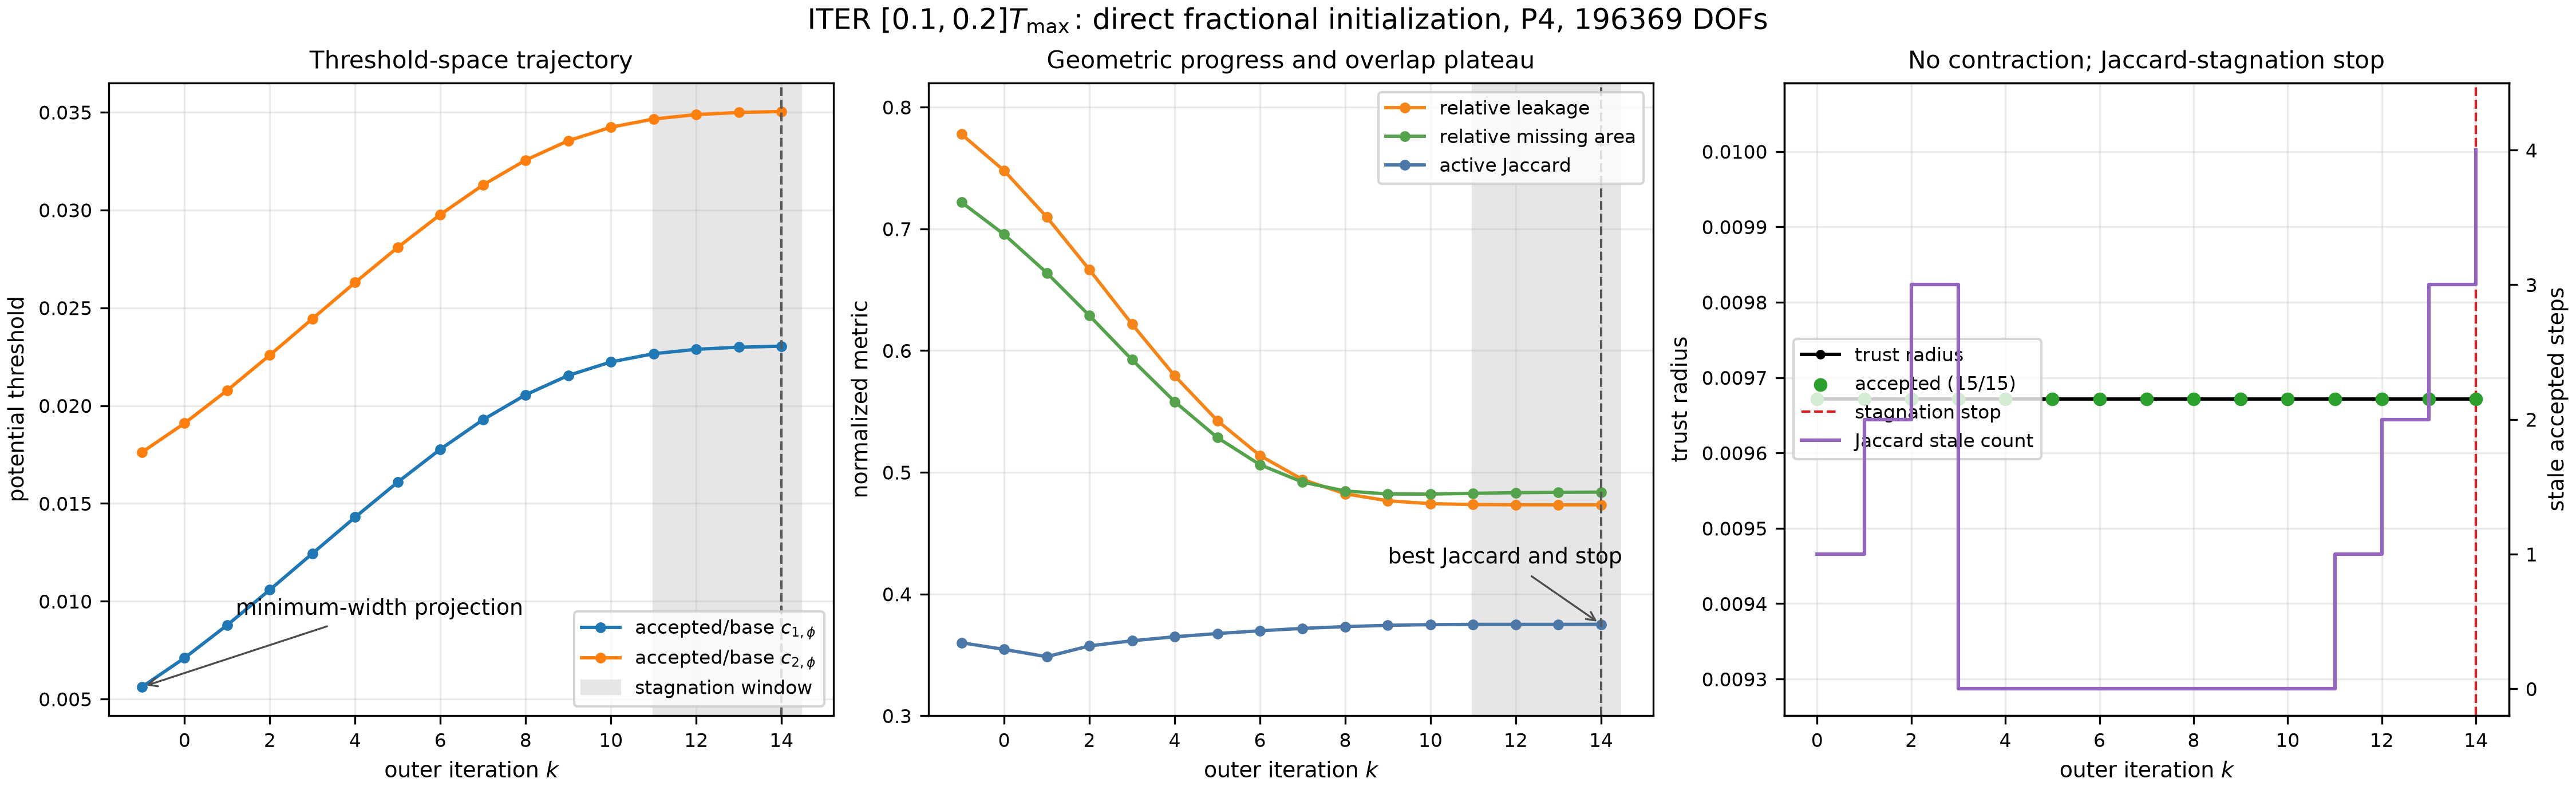
\includegraphics[width=\linewidth]{figures/iter_0p1_0p2_fractional_highdof_optimization_trace.png}
  \caption{Threshold and geometric history for the near-boundary direct
  fractional-initialization run. Left: the raw seed is projected to the
  minimum width before optimization, after which both thresholds translate
  upward together. Centre: leakage and missing area decrease rapidly while
  the hard active Jaccard index first falls and then recovers slowly; the last
  four accepted states fail the configured meaningful-improvement test.
  Right: all 15 trials are accepted, so the trust radius does not contract;
  the terminal four-step stale count triggers termination at $k=14$.}
  \label{fig:iter-fractional-0p1-0p2-trace}
\end{figure}

\begin{table}[htbp]
  \centering
  \caption{Selected fully converged states from the near-boundary direct
  fractional-initialization experiment. $L_{\rm rel}$ and $M_{\rm rel}$
  denote relative leakage and relative missing area. The terminal row is
  simultaneously the stopping state, the exact best-Jaccard state, and the
  state retained for final output.}
  \label{tab:iter-fractional-0p1-0p2}
  \resizebox{\linewidth}{!}{%
  \begin{tabular}{@{}lrrrrrr@{}}
    \toprule
    state & $c_{1,\phi}$ & $c_{2,\phi}$ & residual
      & $L_{\rm rel}$ & $M_{\rm rel}$ & active Jaccard \\
    \midrule
    projected direct seed
      & 0.005613 & 0.017613 & $5.614\times10^{-15}$
      & 0.7777 & 0.7218 & 0.3600 \\
    first accepted state ($k=0$)
      & 0.007098 & 0.019098 & $5.994\times10^{-15}$
      & 0.7478 & 0.6954 & 0.3545 \\
    translated state ($k=8$)
      & 0.020552 & 0.032552 & $7.444\times10^{-15}$
      & 0.4824 & 0.4847 & 0.3732 \\
    stale window begins ($k=11$)
      & 0.022652 & 0.034652 & $7.634\times10^{-15}$
      & 0.4735 & 0.4827 & 0.3751 \\
    stagnation/best state ($k=14$)
      & 0.023035 & 0.035035 & $4.666\times10^{-13}$
      & 0.4732 & 0.4837 & 0.3751 \\
    \bottomrule
  \end{tabular}%
  }
\end{table}

The active Jaccard index began at $0.3600$, fell to $0.3545$ and $0.3485$,
and then recovered to $0.3751$ at $k=11$. Its last four values were
$0.375084$, $0.375076$, $0.375075$, and $0.375132$. The meaningful-improvement
threshold was $10^{-4}+10^{-3}J_{\rm best}$, the configured absolute tolerance
plus its relative contribution, or approximately $4.75\times10^{-4}$ at this
overlap. Consequently, even the new
exact maximum at $k=14$ was too small an improvement to reset the stale
counter. Its fourth step terminated the threshold loop with
\texttt{CONVERGED\_JACCARD\_STAGNATION}. The projected-gradient norm was still
$7.57\times10^1$, so the label again denotes an active-set-overlap plateau
rather than first-order stationarity.

The run marked the best-Jaccard state for restoration, but the exact best was
already the terminal state at $k=14$; restoration therefore did not alter the
thresholds or field. Its residual satisfied the final tolerance, and the
final exact Newton call required zero updates. At this state, active recall
was $0.9979$, active precision was $0.3754$, and the Dice coefficient was
$0.5456$. The reported activity area was $3.1391$ versus target area $3.1723$,
or $98.95\%$ of the target. The nearly complete recall together with the much
lower precision explains why the Jaccard score remained modest despite that
close area total.

The certified core nevertheless had zero area. As in the
$[0.4,0.5]T_{\max}$ experiment, the enforced width was
$\Delta c_\phi=0.012=4\varepsilon_\phi$; with $\kappa=2$, the certified
interval
$[c_{1,\phi}+2\varepsilon_\phi,c_{2,\phi}-2\varepsilon_\phi]$ collapses to a
single level. Thus this is a successful direct nonlinear initialization and
a complete, deliberately terminated reduced-optimization run, but not
certified-subband or first-order geometric convergence. It required no
homotopy, no rejected trial, and no trust-radius contraction. The
noninteractive run took $157.53\,\mathrm{s}$; an otherwise equivalent
plotting run took $185.40\,\mathrm{s}$ and reproduced the reported thresholds
and metrics to roundoff.

\clearpage
\subsection{Small-smoothing high-resolution horseshoe bands}
\label{sec:horseshoe-small-epsilon-highdof}
We finally tested the current reduced optimizer on two horseshoe bands using
the relative smoothing rule
\[
  \varepsilon_\phi=0.01\,(c_{2,\phi}-c_{1,\phi}).
\]
Both runs used the same 24,666-cell mesh, P4 space with 198,529 global degrees
of freedom, quadrature degree 16, eight one-thread MPI ranks, MUMPS, and a
sharp target indicator.  The threshold trust region used the normalized
threshold simplex with the combined Dikin and relative $H^1$ state-pullback
metric.  Thus feasibility and relative changes in every threshold gap were
controlled without inserting a horseshoe-specific width bound.

The initial thresholds were also geometry-derived rather than fitted or
copied from an earlier run.  If $\phi_T$ denotes the Poisson potential of the
sharp target density, the raw pair was
\[
  (c_{1,\phi}^{(0)},c_{2,\phi}^{(0)})
  =(\alpha_1,\alpha_2)\,\|\phi_T\|_{L^\infty},
\]
with $(\alpha_1,\alpha_2)=(0.1,0.2)$ or $(0.4,0.5)$.  Source homotopy then
projected this pair onto an equilibrium branch before the threshold search.
Each homotopy reached $\lambda=1$ in two accepted stages without a rejected
stage.  The resulting experiments are identified by timestamps
\texttt{20260902-155717-304680} and
\texttt{20260902-155101-964442}, respectively.

Table~\ref{tab:horseshoe-small-epsilon-highdof} reports the restored state
with the largest \emph{observed} hard active-set Jaccard score in each run.
Here $L_{\mathrm{rel}}$ and $M_{\mathrm{rel}}$ are relative leakage and
missing area.  These data do not supply an upper bound on the attainable
Jaccard score and therefore do not establish threshold-space convergence.

\begin{table}[tbp]
  \centering
  \resizebox{\linewidth}{!}{%
  \begin{tabular}{lcc}
    \toprule
    Quantity & $[0.1,0.2]T_{\max}$ & $[0.4,0.5]T_{\max}$ \\
    \midrule
    $\|\phi_T\|_{L^\infty}$
      & $2.698604\times10^{-3}$ & $6.096742\times10^{-3}$ \\
    Initial $(c_{1,\phi},c_{2,\phi})$
      & $(2.698604,5.397209)\times10^{-4}$
      & $(2.438697,3.048371)\times10^{-3}$ \\
    Selected $(c_{1,\phi},c_{2,\phi})$
      & $(4.869176,7.656884)\times10^{-4}$
      & $(2.904630,3.488980)\times10^{-3}$ \\
    Selected $\Delta c_\phi$
      & $2.787707\times10^{-4}$ & $5.843498\times10^{-4}$ \\
    Hard Jaccard, seed $\to$ selected
      & $0.4705\to0.5971$ & $0.3568\to0.4524$ \\
    Soft Jaccard at selected state
      & $0.5504$ & $0.4211$ \\
    $(L_{\mathrm{rel}},M_{\mathrm{rel}})$
      & $(0.2834,0.2936)$ & $(0.5288,0.3563)$ \\
    Active recall / precision / Dice
      & $0.8077/0.6961/0.7478$ & $0.7393/0.5382/0.6230$ \\
    Certified area / target area
      & $0.8423$ & $0.9980$ \\
    Certified leakage / target area
      & $0.1964$ & $0.4030$ \\
    Accepted threshold steps
      & $10$ & $9$ \\
    Selected residual
      & $1.20\times10^{-16}$ & $5.03\times10^{-16}$ \\
    \bottomrule
  \end{tabular}}
  \caption{High-resolution horseshoe tests with
  $\varepsilon_\phi/\Delta c_\phi=0.01$.  ``Selected'' means the restored
  state with the largest hard Jaccard value observed during that run, not a
  certified global maximizer.}
  \label{tab:horseshoe-small-epsilon-highdof}
\end{table}

\paragraph{Near-boundary band $[0.1,0.2]T_{\max}$.}
The search moved the threshold center by about $54.7\%$ while changing the
window width by only $3.3\%$.  This is precisely the kind of anisotropic
motion that a center/width interpretation makes visible: most of the useful
change was translation of the band, not collapse or expansion of its width.
The hard Jaccard score attained its observed maximum at accepted state
$k=10$.  Four later accepted states failed to exceed it, so the loop stopped
with \texttt{STOPPED\_JACCARD\_STAGNATION} and restored $k=10$.  The final
exact Newton projection required no update because the restored state already
satisfied the residual tolerance.

\paragraph{Interior band $[0.4,0.5]T_{\max}$.}
Here the selected center increased by about $16.5\%$ and the width decreased
by about $4.2\%$.  The largest observed hard Jaccard value occurred at
accepted state $k=12$.  Subsequent accepted states changed the smooth
objective slightly but did not improve that hard-overlap record; after four
stale accepted states the loop stopped and restored $k=12$.  This separation
between the smooth objective and the hard diagnostic is expected and is why
the code stores the best observed hard-overlap state independently of the
terminal state.

The smaller smoothing left a nonempty certified potential interval in both
tests: for $\kappa=2$, its potential width is $96\%$ of
$\Delta c_\phi$.  This removes the artificial certified-core collapse seen
when $\Delta c_\phi=4\varepsilon_\phi$ in the older ITER examples.  It does
not, by itself, guarantee low geometric leakage, as the certified leakage
column in Table~\ref{tab:horseshoe-small-epsilon-highdof} makes clear.

The rescue-only energy primer was rarely active.  The near-boundary run made
one primer call and retained one accepted step; its next candidate was
discarded because the $H^{-1}$ residual failed to improve materially.  The
interior run made two calls and retained no primer step: one was stopped by
the branch-loss guard and the other by the residual-progress guard.  Hence
the reported states were determined primarily by Newton and the threshold
trust region rather than by a long energy-descent phase.

Generalized eigenvalue diagnostics also rule out undamped Picard iteration as
a replacement for the safeguarded primer in these two states.  At the
selected near-boundary equilibrium the measured Picard interval was
$[-33.22,0.757]$; at the selected interior equilibrium it was
$[-59.89,0.827]$.  In both cases the upper endpoint below one is consistent
with a locally positive energy Hessian in the measured subspace, while the
large negative endpoint gives a Picard spectral-radius bound far above one.
Thus the equilibria can be local energy minima even though the raw fixed-point
map is not locally contractive.  Damped, line-searched energy steps remain the
safer rescue mechanism.

We classify these as completed, branch-preserving PDE solves with improved
observed overlap and nonempty certified cores.  We do not call the threshold
search converged: it stopped because the best observed hard Jaccard score
stagnated.  The two executions overlapped in wall-clock time, so their total
times are not used as comparative performance measurements.
